%%
%% This is file `sample-sigconf.tex',
%% generated with the docstrip utility.
%%
%% The original source files were:
%%
%% samples.dtx  (with options: `all,proceedings,bibtex,sigconf')
%% 
%% IMPORTANT NOTICE:
%% 
%% For the copyright see the source file.
%% 
%% Any modified versions of this file must be renamed
%% with new filenames distinct from sample-sigconf.tex.
%% 
%% For distribution of the original source see the terms
%% for copying and modification in the file samples.dtx.
%% 
%% This generated file may be distributed as long as the
%% original source files, as listed above, are part of the
%% same distribution. (The sources need not necessarily be
%% in the same archive or directory.)
%%
%%
%% Commands for TeXCount
%TC:macro \cite [option:text,text]
%TC:macro \citep [option:text,text]
%TC:macro \citet [option:text,text]
%TC:envir table 0 1
%TC:envir table* 0 1
%TC:envir tabular [ignore] word
%TC:envir displaymath 0 word
%TC:envir math 0 word
%TC:envir comment 0 0
%%
%%
%% The first command in your LaTeX source must be the \documentclass
%% command.
%%
%% For submission and review of your manuscript please change the
%% command to \documentclass[manuscript, screen, review]{acmart}.
%%
%% When submitting camera ready or to TAPS, please change the command
%% to \documentclass[sigconf]{acmart} or whichever template is required
%% for your publication.
%%
%%
%\documentclass[sigconf, screen, review]{acmart}
\documentclass[sigplan, dvipsnames, screen, nonacm]{acmart}

%%
%% \BibTeX command to typeset BibTeX logo in the docs
\AtBeginDocument{%
  \providecommand\BibTeX{{%
    Bib\TeX}}}

%% Rights management information.  This information is sent to you
%% when you complete the rights form.  These commands have SAMPLE
%% values in them; it is your responsibility as an author to replace
%% the commands and values with those provided to you when you
%% complete the rights form.
\setcopyright{none} 
%\setcopyright{acmlicensed}
\copyrightyear{2024}
\acmYear{2024}
\acmDOI{XXXXXXX.XXXXXXX}

%% These commands are for a PROCEEDINGS abstract or paper.
\acmConference['ISCA 2025']{The 52nd IEEE/ACM International Symposium on Computer Architecture}{June 21--25, 2025}{Tokyo, Japan}
%\acmConference[]{}{}{}
%%
%%  Uncomment \acmBooktitle if the title of the proceedings is different
%%  from ``Proceedings of ...''!
%%
%%\acmBooktitle{Woodstock '18: ACM Symposium on Neural Gaze Detection,
%%  June 03--05, 2018, Woodstock, NY}
%\acmISBN{978-1-4503-XXXX-X/18/06}


%%
%% Submission ID.
%% Use this when submitting an article to a sponsored event. You'll
%% receive a unique submission ID from the organizers
%% of the event, and this ID should be used as the parameter to this command.
%%\acmSubmissionID{123-A56-BU3}

%%
%% For managing citations, it is recommended to use bibliography
%% files in BibTeX format.
%%
%% You can then either use BibTeX with the ACM-Reference-Format style,
%% or BibLaTeX with the acmnumeric or acmauthoryear sytles, that include
%% support for advanced citation of software artefact from the
%% biblatex-software package, also separately available on CTAN.
%%
%% Look at the sample-*-biblatex.tex files for templates showcasing
%% the biblatex styles.
%%

%%
%% The majority of ACM publications use numbered citations and
%% references.  The command \citestyle{authoryear} switches to the
%% "author year" style.
%%
%% If you are preparing content for an event
%% sponsored by ACM SIGGRAPH, you must use the "author year" style of
%% citations and references.
%% Uncommenting
%% the next command will enable that style.
%%\citestyle{acmauthoryear}
\settopmatter{printfolios=false}
\settopmatter{printacmref=false}
\renewcommand\footnotetextcopyrightpermission[1]{}%
% Common packages
\usepackage[utf8]{inputenc} % allow utf-8 input
\usepackage[T1]{fontenc}    % use 8-bit T1 fonts
\usepackage{microtype,inconsolata}
\usepackage{times,latexsym}
\usepackage{graphicx} \graphicspath{{figures/}}
\usepackage{amsmath,amssymb,mathabx,mathtools,amsthm,nicefrac}
% \usepackage{algorithmic}
\usepackage[linesnumbered,ruled,vlined]{algorithm2e}
\usepackage{acronym}
\usepackage{enumitem}
%\usepackage[pagebackref,breaklinks,colorlinks]{hyperref}
\usepackage{balance}
\usepackage{xspace}
\usepackage{setspace}
\usepackage[skip=3pt,font=small]{subcaption}
\usepackage[skip=3pt,font=small]{caption}
%\usepackage[dvipsnames,svgnames,x11names,table]{xcolor}
\usepackage[capitalise,noabbrev,nameinlink]{cleveref}
\usepackage{booktabs,tabularx,colortbl,multirow,multicol,array,makecell,tabularray}
\usepackage{overpic,wrapfig}
\usepackage[misc]{ifsym}
\usepackage{pifont}
\usepackage{diagbox}


% Handy shorthand
\makeatletter
\DeclareRobustCommand\onedot{\futurelet\@let@token\@onedot}
\def\@onedot{\ifx\@let@token.\else.\null\fi\xspace}
\def\eg{\emph{e.g}\onedot} 
\def\Eg{\emph{E.g}\onedot}
\def\ie{\emph{i.e}\onedot} 
\def\Ie{\emph{I.e}\onedot}
\def\cf{\emph{c.f}\onedot} 
\def\Cf{\emph{C.f}\onedot}
\def\etc{\emph{etc}\onedot} 
\def\vs{\emph{vs}\onedot}
\def\aka{a.k.a\onedot}
\def\wrt{w.r.t\onedot} 
\def\dof{d.o.f\onedot}
\def\etal{\emph{et al}\onedot}
\makeatother

% Handy math ops
%\DeclareMathOperator*{\argmax}{arg\,max}
%\DeclareMathOperator*{\argmin}{arg\,min}
\DeclareMathOperator*{\kl}{KL}
\newcommand\energy{\mathcal{E}}
\newcommand{\norm}[1]{\left\Vert #1 \right\Vert}

% Handy table symbols
\newcommand{\cmark}{\ding{51}}%
\newcommand{\xmark}{\ding{55}}%

% Spacing
\frenchspacing
\makeatletter
\renewcommand{\paragraph}{%
  \@startsection{paragraph}{4}%
  {\z@}{0ex \@plus 0ex \@minus 0ex}{-1em}%
  {\hskip0em\normalfont\normalsize\bfseries}%
}
\makeatother

% Clever references
\crefname{algorithm}{Alg.}{Algs.}
\Crefname{algocf}{Algorithm}{Algorithms}
\crefname{section}{Sec.}{Secs.}
\Crefname{section}{Section}{Sections}
\crefname{table}{Tab.}{Tabs.}
\Crefname{table}{Table}{Tables}
\crefname{figure}{Fig.}{Figs.}
\Crefname{figure}{Figure}{Figures}
\crefname{equation}{Eq.}{Eqs.}
\Crefname{equation}{Equation}{Equations}
\crefname{appendix}{Appx.}{Appxs.}
\Crefname{appendix}{Appendix}{Appendices}

% Handy Colors
\definecolor{gblue}{HTML}{4285F4}
\definecolor{gred}{HTML}{DB4437}
\definecolor{ggreen}{HTML}{0F9D58}

\hypersetup{
  %citecolor=gray %Colour of citations
}

% Spacing
% \frenchspacing
% \medmuskip=2mu   % reduce spacing around binary operators
% \thickmuskip=3mu % reduce spacing around relational operators
% \setlength{\abovedisplayskip}{3pt}
% \setlength{\belowdisplayskip}{3pt}
% \setlength{\abovecaptionskip}{3pt}
% \setlength{\belowcaptionskip}{3pt}
% \setlength\floatsep{0.5\baselineskip plus 3pt minus 2pt}
% \setlength\textfloatsep{0.5\baselineskip plus 3pt minus 2pt}
% \setlength\dbltextfloatsep{0.5\baselineskip plus 3pt minus 2pt}
% \setlength\intextsep{0.5\baselineskip plus 3pt minus 2pt}

\newcolumntype{P}[1]{>{\centering\arraybackslash}p{#1}}
\newcolumntype{M}[1]{>{\centering\arraybackslash}m{#1}}

\acrodef{metaicl-w}[Minnow]{Meta-training for IN-context learNing Of Words}
\acrodef{metaicl}[MetaICL]{Meta-training for In-Context Learning}
\acrodef{icl}[ICL]{in-context learning}
\author{%
  Wentao Wang$^1$ \hspace{1em} Guangyuan Jiang$^2$ \hspace{1em} Tal Linzen$^1$ \hspace{1em} Brenden M.\ Lake$^1$ \\
  $^1$New York University \hspace{1em} $^2$Peking University \\
  \texttt{\{ww2135, linzen, brenden\}@nyu.edu} \hspace{1em} \texttt{jgy@stu.pku.edu.cn}
}
%\pagestyle{empty}   % Removes headers/footers from every page
\pagestyle{plain}

%%
%% end of the preamble, start of the body of the document source.
\begin{document}

%%
%% The "title" command has an optional parameter,
%% allowing the author to define a "short title" to be used in page headers.
\title{Nexus Machine: An Active Message Inspired Reconfigurable Architecture for Irregular Workloads}
%\subtitle{\normalsize{ISCA 2025 Submission
%    \textbf{\#415} -- Confidential Draft -- Do NOT Distribute!!}}
%%
%% The "author" command and its associated commands are used to define
%% the authors and their affiliations.
%% Of note is the shared affiliation of the first two authors, and the
%% "authornote" and "authornotemark" commands
%% used to denote shared contribution to the research.
%\author{\normalsize{ISCA 2025 Submission
 %   \textbf{\#NaN} -- Confidential Draft -- Do NOT Distribute!!}}

%%
%% By default, the full list of authors will be used in the page
%% headers. Often, this list is too long, and will overlap
%% other information printed in the page headers. This command allows
%% the author to define a more concise list
%% of authors' names for this purpose.
\author{Rohan Juneja}
\email{rohan@comp.nus.edu.sg}
\affiliation{%
  \institution{National University of Singapore}
  \country{Singapore}
}

\author{Pranav Dangi}
\email{dangi@comp.nus.edu.sg}
\affiliation{%
  \institution{National University of Singapore}
  \country{Singapore}
}

\author{Thilini Kaushalya Bandara}
\email{thilini@comp.nus.edu.sg}
\affiliation{%
  \institution{National University of Singapore}
  \country{Singapore}
}

\author{Zhaoying Li}
\email{zhaoying@comp.nus.edu.sg}
\affiliation{%
  \institution{National University of Singapore}
  \country{Singapore}
}

\author{Tulika Mitra}
\email{tulika@comp.nus.edu.sg}
\affiliation{%
  \institution{National University of Singapore}
  \country{Singapore}
}

\author{Li-Shiuan Peh}
\email{peh@comp.nus.edu.sg}
\affiliation{%
  \institution{National University of Singapore}
  \country{Singapore}
}


%%
%% The abstract is a short summary of the work to be presented in the
%% article.
\begin{abstract}
Modern reconfigurable architectures are increasingly favored for resource-constrained edge devices as they balance high performance, energy efficiency, and programmability well. 
%{\color{blue}Unlike FPGAs, which reconfigure at the LUT level, CGRAs allow reconfigurability at the instruction level by directly reconfiguring ALUs.}
However, their proficiency in handling regular compute patterns constrains their effectiveness in executing irregular workloads, such as sparse linear algebra and graph analytics with unpredictable access patterns and control flow.

To address this limitation, we introduce the \textit{Nexus Machine}, a novel reconfigurable architecture consisting of a PE array designed to efficiently handle irregularity by distributing sparse tensors across the fabric and employing active messages that morph instructions based on dynamic control flow. 
As the inherent irregularity in workloads can lead to high load imbalance among different Processing Elements (PEs), \textit{Nexus Machine} deploys and executes instructions en-route on idle PEs at run-time. 
Thus, unlike traditional reconfigurable architectures with only static instructions within each PE, \textit{Nexus Machine} brings dynamic control to the idle compute units, mitigating load imbalance and enhancing overall performance.
Our experiments demonstrate that \textit{Nexus Machine} achieves 1.5x performance gain compared to state-of-the-art (SOTA) reconfigurable architectures, within the same power budget and area. \textit{Nexus Machine} also achieves 1.6x higher fabric utilization, in contrast to SOTA architectures..
\end{abstract}

%%
%% The code below is generated by the tool at http://dl.acm.org/ccs.cfm.
%% Please copy and paste the code instead of the example below.
%%
%\begin{CCSXML}
%<ccs2012>
% <concept>
%  <concept_id>00000000.0000000.0000000</concept_id>
%  <concept_desc>Do Not Use This Code, Generate the Correct Terms for Your Paper</concept_desc>
%  <concept_significance>500</concept_significance>
% </concept>
% <concept>
%  %<concept_id>00000000.00000000.00000000</concept_id>
%  <concept_desc>Do Not Use This Code, Generate the Correct Terms for Your Paper</concept_desc>
%  <concept_significance>300</concept_significance>
% </concept>
% <concept>
%  %<concept_id>00000000.00000000.00000000</concept_id>
%  <concept_desc>Do Not Use This Code, Generate the Correct Terms for Your Paper</concept_desc>
%  <concept_significance>100</concept_significance>
% </concept>
% <concept>
 % <concept_id>00000000.00000000.00000000</concept_id>
%  <concept_desc>Do Not Use This Code, Generate the Correct Terms for Your Paper</concept_desc>
%  <concept_significance>100</concept_significance>
% </concept>
%</ccs2012>
%\end{CCSXML}

%\ccsdesc[500]{Do Not Use This Code~Generate the Correct Terms for Your Paper}
%\ccsdesc[300]{Do Not Use This Code~Generate the Correct Terms for Your Paper}
%\ccsdesc{Do Not Use This Code~Generate the Correct Terms for Your Paper}
%\ccsdesc[100]{Do Not Use This Code~Generate the Correct Terms for Your Paper}

%%
%% Keywords. The author(s) should pick words that accurately describe
%% the work being presented. Separate the keywords with commas.
\keywords{Reconfigurable, Sparsity, Graph, Active Messages}

\maketitle


\section{Introduction}
\label{sec:introduction}
The business processes of organizations are experiencing ever-increasing complexity due to the large amount of data, high number of users, and high-tech devices involved \cite{martin2021pmopportunitieschallenges, beerepoot2023biggestbpmproblems}. This complexity may cause business processes to deviate from normal control flow due to unforeseen and disruptive anomalies \cite{adams2023proceddsriftdetection}. These control-flow anomalies manifest as unknown, skipped, and wrongly-ordered activities in the traces of event logs monitored from the execution of business processes \cite{ko2023adsystematicreview}. For the sake of clarity, let us consider an illustrative example of such anomalies. Figure \ref{FP_ANOMALIES} shows a so-called event log footprint, which captures the control flow relations of four activities of a hypothetical event log. In particular, this footprint captures the control-flow relations between activities \texttt{a}, \texttt{b}, \texttt{c} and \texttt{d}. These are the causal ($\rightarrow$) relation, concurrent ($\parallel$) relation, and other ($\#$) relations such as exclusivity or non-local dependency \cite{aalst2022pmhandbook}. In addition, on the right are six traces, of which five exhibit skipped, wrongly-ordered and unknown control-flow anomalies. For example, $\langle$\texttt{a b d}$\rangle$ has a skipped activity, which is \texttt{c}. Because of this skipped activity, the control-flow relation \texttt{b}$\,\#\,$\texttt{d} is violated, since \texttt{d} directly follows \texttt{b} in the anomalous trace.
\begin{figure}[!t]
\centering
\includegraphics[width=0.9\columnwidth]{images/FP_ANOMALIES.png}
\caption{An example event log footprint with six traces, of which five exhibit control-flow anomalies.}
\label{FP_ANOMALIES}
\end{figure}

\subsection{Control-flow anomaly detection}
Control-flow anomaly detection techniques aim to characterize the normal control flow from event logs and verify whether these deviations occur in new event logs \cite{ko2023adsystematicreview}. To develop control-flow anomaly detection techniques, \revision{process mining} has seen widespread adoption owing to process discovery and \revision{conformance checking}. On the one hand, process discovery is a set of algorithms that encode control-flow relations as a set of model elements and constraints according to a given modeling formalism \cite{aalst2022pmhandbook}; hereafter, we refer to the Petri net, a widespread modeling formalism. On the other hand, \revision{conformance checking} is an explainable set of algorithms that allows linking any deviations with the reference Petri net and providing the fitness measure, namely a measure of how much the Petri net fits the new event log \cite{aalst2022pmhandbook}. Many control-flow anomaly detection techniques based on \revision{conformance checking} (hereafter, \revision{conformance checking}-based techniques) use the fitness measure to determine whether an event log is anomalous \cite{bezerra2009pmad, bezerra2013adlogspais, myers2018icsadpm, pecchia2020applicationfailuresanalysispm}. 

The scientific literature also includes many \revision{conformance checking}-independent techniques for control-flow anomaly detection that combine specific types of trace encodings with machine/deep learning \cite{ko2023adsystematicreview, tavares2023pmtraceencoding}. Whereas these techniques are very effective, their explainability is challenging due to both the type of trace encoding employed and the machine/deep learning model used \cite{rawal2022trustworthyaiadvances,li2023explainablead}. Hence, in the following, we focus on the shortcomings of \revision{conformance checking}-based techniques to investigate whether it is possible to support the development of competitive control-flow anomaly detection techniques while maintaining the explainable nature of \revision{conformance checking}.
\begin{figure}[!t]
\centering
\includegraphics[width=\columnwidth]{images/HIGH_LEVEL_VIEW.png}
\caption{A high-level view of the proposed framework for combining \revision{process mining}-based feature extraction with dimensionality reduction for control-flow anomaly detection.}
\label{HIGH_LEVEL_VIEW}
\end{figure}

\subsection{Shortcomings of \revision{conformance checking}-based techniques}
Unfortunately, the detection effectiveness of \revision{conformance checking}-based techniques is affected by noisy data and low-quality Petri nets, which may be due to human errors in the modeling process or representational bias of process discovery algorithms \cite{bezerra2013adlogspais, pecchia2020applicationfailuresanalysispm, aalst2016pm}. Specifically, on the one hand, noisy data may introduce infrequent and deceptive control-flow relations that may result in inconsistent fitness measures, whereas, on the other hand, checking event logs against a low-quality Petri net could lead to an unreliable distribution of fitness measures. Nonetheless, such Petri nets can still be used as references to obtain insightful information for \revision{process mining}-based feature extraction, supporting the development of competitive and explainable \revision{conformance checking}-based techniques for control-flow anomaly detection despite the problems above. For example, a few works outline that token-based \revision{conformance checking} can be used for \revision{process mining}-based feature extraction to build tabular data and develop effective \revision{conformance checking}-based techniques for control-flow anomaly detection \cite{singh2022lapmsh, debenedictis2023dtadiiot}. However, to the best of our knowledge, the scientific literature lacks a structured proposal for \revision{process mining}-based feature extraction using the state-of-the-art \revision{conformance checking} variant, namely alignment-based \revision{conformance checking}.

\subsection{Contributions}
We propose a novel \revision{process mining}-based feature extraction approach with alignment-based \revision{conformance checking}. This variant aligns the deviating control flow with a reference Petri net; the resulting alignment can be inspected to extract additional statistics such as the number of times a given activity caused mismatches \cite{aalst2022pmhandbook}. We integrate this approach into a flexible and explainable framework for developing techniques for control-flow anomaly detection. The framework combines \revision{process mining}-based feature extraction and dimensionality reduction to handle high-dimensional feature sets, achieve detection effectiveness, and support explainability. Notably, in addition to our proposed \revision{process mining}-based feature extraction approach, the framework allows employing other approaches, enabling a fair comparison of multiple \revision{conformance checking}-based and \revision{conformance checking}-independent techniques for control-flow anomaly detection. Figure \ref{HIGH_LEVEL_VIEW} shows a high-level view of the framework. Business processes are monitored, and event logs obtained from the database of information systems. Subsequently, \revision{process mining}-based feature extraction is applied to these event logs and tabular data input to dimensionality reduction to identify control-flow anomalies. We apply several \revision{conformance checking}-based and \revision{conformance checking}-independent framework techniques to publicly available datasets, simulated data of a case study from railways, and real-world data of a case study from healthcare. We show that the framework techniques implementing our approach outperform the baseline \revision{conformance checking}-based techniques while maintaining the explainable nature of \revision{conformance checking}.

In summary, the contributions of this paper are as follows.
\begin{itemize}
    \item{
        A novel \revision{process mining}-based feature extraction approach to support the development of competitive and explainable \revision{conformance checking}-based techniques for control-flow anomaly detection.
    }
    \item{
        A flexible and explainable framework for developing techniques for control-flow anomaly detection using \revision{process mining}-based feature extraction and dimensionality reduction.
    }
    \item{
        Application to synthetic and real-world datasets of several \revision{conformance checking}-based and \revision{conformance checking}-independent framework techniques, evaluating their detection effectiveness and explainability.
    }
\end{itemize}

The rest of the paper is organized as follows.
\begin{itemize}
    \item Section \ref{sec:related_work} reviews the existing techniques for control-flow anomaly detection, categorizing them into \revision{conformance checking}-based and \revision{conformance checking}-independent techniques.
    \item Section \ref{sec:abccfe} provides the preliminaries of \revision{process mining} to establish the notation used throughout the paper, and delves into the details of the proposed \revision{process mining}-based feature extraction approach with alignment-based \revision{conformance checking}.
    \item Section \ref{sec:framework} describes the framework for developing \revision{conformance checking}-based and \revision{conformance checking}-independent techniques for control-flow anomaly detection that combine \revision{process mining}-based feature extraction and dimensionality reduction.
    \item Section \ref{sec:evaluation} presents the experiments conducted with multiple framework and baseline techniques using data from publicly available datasets and case studies.
    \item Section \ref{sec:conclusions} draws the conclusions and presents future work.
\end{itemize}
\section{Bellman Error Centering}

Centering operator $\mathcal{C}$ for a variable $x(s)$ is defined as follows:
\begin{equation}
\mathcal{C}x(s)\dot{=} x(s)-\mathbb{E}[x(s)]=x(s)-\sum_s{d_{s}x(s)},
\end{equation} 
where $d_s$ is the probability of $s$.
In vector form,
\begin{equation}
\begin{split}
\mathcal{C}\bm{x} &= \bm{x}-\mathbb{E}[x]\bm{1}\\
&=\bm{x}-\bm{x}^{\top}\bm{d}\bm{1},
\end{split}
\end{equation} 
where $\bm{1}$ is an all-ones vector.
For any vector $\bm{x}$ and $\bm{y}$ with a same distribution $\bm{d}$,
we have
\begin{equation}
\begin{split}
\mathcal{C}(\bm{x}+\bm{y})&=(\bm{x}+\bm{y})-(\bm{x}+\bm{y})^{\top}\bm{d}\bm{1}\\
&=\bm{x}-\bm{x}^{\top}\bm{d}\bm{1}+\bm{y}-\bm{y}^{\top}\bm{d}\bm{1}\\
&=\mathcal{C}\bm{x}+\mathcal{C}\bm{y}.
\end{split}
\end{equation}
\subsection{Revisit Reward Centering}


The update (\ref{src3}) is an unbiased estimate of the average reward
with  appropriate learning rate $\beta_t$ conditions.
\begin{equation}
\bar{r}_{t}\approx \lim_{n\rightarrow\infty}\frac{1}{n}\sum_{t=1}^n\mathbb{E}_{\pi}[r_t].
\end{equation}
That is 
\begin{equation}
r_t-\bar{r}_{t}\approx r_t-\lim_{n\rightarrow\infty}\frac{1}{n}\sum_{t=1}^n\mathbb{E}_{\pi}[r_t]= \mathcal{C}r_t.
\end{equation}
Then, the simple reward centering can be rewrited as:
\begin{equation}
V_{t+1}(s_t)=V_{t}(s_t)+\alpha_t [\mathcal{C}r_{t+1}+\gamma V_{t}(s_{t+1})-V_t(s_t)].
\end{equation}
Therefore, the simple reward centering is, in a strict sense, reward centering.

By definition of $\bar{\delta}_t=\delta_t-\bar{r}_{t}$,
let rewrite the update rule of the value-based reward centering as follows:
\begin{equation}
V_{t+1}(s_t)=V_{t}(s_t)+\alpha_t \rho_t (\delta_t-\bar{r}_{t}),
\end{equation}
where $\bar{r}_{t}$ is updated as:
\begin{equation}
\bar{r}_{t+1}=\bar{r}_{t}+\beta_t \rho_t(\delta_t-\bar{r}_{t}).
\label{vrc3}
\end{equation}
The update (\ref{vrc3}) is an unbiased estimate of the TD error
with  appropriate learning rate $\beta_t$ conditions.
\begin{equation}
\bar{r}_{t}\approx \mathbb{E}_{\pi}[\delta_t].
\end{equation}
That is 
\begin{equation}
\delta_t-\bar{r}_{t}\approx \mathcal{C}\delta_t.
\end{equation}
Then, the value-based reward centering can be rewrited as:
\begin{equation}
V_{t+1}(s_t)=V_{t}(s_t)+\alpha_t \rho_t \mathcal{C}\delta_t.
\label{tdcentering}
\end{equation}
Therefore, the value-based reward centering is no more,
 in a strict sense, reward centering.
It is, in a strict sense, \textbf{Bellman error centering}.

It is worth noting that this understanding is crucial, 
as designing new algorithms requires leveraging this concept.


\subsection{On the Fixpoint Solution}

The update rule (\ref{tdcentering}) is a stochastic approximation
of the following update:
\begin{equation}
\begin{split}
V_{t+1}&=V_{t}+\alpha_t [\bm{\mathcal{T}}^{\pi}\bm{V}-\bm{V}-\mathbb{E}[\delta]\bm{1}]\\
&=V_{t}+\alpha_t [\bm{\mathcal{T}}^{\pi}\bm{V}-\bm{V}-(\bm{\mathcal{T}}^{\pi}\bm{V}-\bm{V})^{\top}\bm{d}_{\pi}\bm{1}]\\
&=V_{t}+\alpha_t [\mathcal{C}(\bm{\mathcal{T}}^{\pi}\bm{V}-\bm{V})].
\end{split}
\label{tdcenteringVector}
\end{equation}
If update rule (\ref{tdcenteringVector}) converges, it is expected that
$\mathcal{C}(\mathcal{T}^{\pi}V-V)=\bm{0}$.
That is 
\begin{equation}
    \begin{split}
    \mathcal{C}\bm{V} &= \mathcal{C}\bm{\mathcal{T}}^{\pi}\bm{V} \\
    &= \mathcal{C}(\bm{R}^{\pi} + \gamma \mathbb{P}^{\pi} \bm{V}) \\
    &= \mathcal{C}\bm{R}^{\pi} + \gamma \mathcal{C}\mathbb{P}^{\pi} \bm{V} \\
    &= \mathcal{C}\bm{R}^{\pi} + \gamma (\mathbb{P}^{\pi} \bm{V} - (\mathbb{P}^{\pi} \bm{V})^{\top} \bm{d_{\pi}} \bm{1}) \\
    &= \mathcal{C}\bm{R}^{\pi} + \gamma (\mathbb{P}^{\pi} \bm{V} - \bm{V}^{\top} (\mathbb{P}^{\pi})^{\top} \bm{d_{\pi}} \bm{1}) \\  % 修正双重上标
    &= \mathcal{C}\bm{R}^{\pi} + \gamma (\mathbb{P}^{\pi} \bm{V} - \bm{V}^{\top} \bm{d_{\pi}} \bm{1}) \\
    &= \mathcal{C}\bm{R}^{\pi} + \gamma (\mathbb{P}^{\pi} \bm{V} - \bm{V}^{\top} \bm{d_{\pi}} \mathbb{P}^{\pi} \bm{1}) \\
    &= \mathcal{C}\bm{R}^{\pi} + \gamma (\mathbb{P}^{\pi} \bm{V} - \mathbb{P}^{\pi} \bm{V}^{\top} \bm{d_{\pi}} \bm{1}) \\
    &= \mathcal{C}\bm{R}^{\pi} + \gamma \mathbb{P}^{\pi} (\bm{V} - \bm{V}^{\top} \bm{d_{\pi}} \bm{1}) \\
    &= \mathcal{C}\bm{R}^{\pi} + \gamma \mathbb{P}^{\pi} \mathcal{C}\bm{V} \\
    &\dot{=} \bm{\mathcal{T}}_c^{\pi} \mathcal{C}\bm{V},
    \end{split}
    \label{centeredfixpoint}
    \end{equation}
where we defined $\bm{\mathcal{T}}_c^{\pi}$ as a centered Bellman operator.
We call equation (\ref{centeredfixpoint}) as centered Bellman equation.
And it is \textbf{centered fixpoint}.

For linear value function approximation, let define
\begin{equation}
\mathcal{C}\bm{V}_{\bm{\theta}}=\bm{\Pi}\bm{\mathcal{T}}_c^{\pi}\mathcal{C}\bm{V}_{\bm{\theta}}.
\label{centeredTDfixpoint}
\end{equation}
We call equation (\ref{centeredTDfixpoint}) as \textbf{centered TD fixpoint}.

\subsection{On-policy and Off-policy Centered TD Algorithms
with Linear Value Function Approximation}
Given the above centered TD fixpoint,
 mean squared centered Bellman error (MSCBE), is proposed as follows:
\begin{align*}
    \label{argminMSBEC}
 &\arg \min_{{\bm{\theta}}}\text{MSCBE}({\bm{\theta}}) \\
 &= \arg \min_{{\bm{\theta}}} \|\bm{\mathcal{T}}_c^{\pi}\mathcal{C}\bm{V}_{\bm{{\bm{\theta}}}}-\mathcal{C}\bm{V}_{\bm{{\bm{\theta}}}}\|_{\bm{D}}^2\notag\\
 &=\arg \min_{{\bm{\theta}}} \|\bm{\mathcal{T}}^{\pi}\bm{V}_{\bm{{\bm{\theta}}}} - \bm{V}_{\bm{{\bm{\theta}}}}-(\bm{\mathcal{T}}^{\pi}\bm{V}_{\bm{{\bm{\theta}}}} - \bm{V}_{\bm{{\bm{\theta}}}})^{\top}\bm{d}\bm{1}\|_{\bm{D}}^2\notag\\
 &=\arg \min_{{\bm{\theta}},\omega} \| \bm{\mathcal{T}}^{\pi}\bm{V}_{\bm{{\bm{\theta}}}} - \bm{V}_{\bm{{\bm{\theta}}}}-\omega\bm{1} \|_{\bm{D}}^2\notag,
\end{align*}
where $\omega$ is is used to estimate the expected value of the Bellman error.
% where $\omega$ is used to estimate $\mathbb{E}[\delta]$, $\omega \doteq \mathbb{E}[\mathbb{E}[\delta_t|S_t]]=\mathbb{E}[\delta]$ and $\delta_t$ is the TD error as follows:
% \begin{equation}
% \delta_t = r_{t+1}+\gamma
% {\bm{\theta}}_t^{\top}\bm{{\bm{\phi}}}_{t+1}-{\bm{\theta}}_t^{\top}\bm{{\bm{\phi}}}_t.
% \label{delta}
% \end{equation}
% $\mathbb{E}[\delta_t|S_t]$ is the Bellman error, and $\mathbb{E}[\mathbb{E}[\delta_t|S_t]]$ represents the expected value of the Bellman error.
% If $X$ is a random variable and $\mathbb{E}[X]$ is its expected value, then $X-\mathbb{E}[X]$ represents the centered form of $X$. 
% Therefore, we refer to $\mathbb{E}[\delta_t|S_t]-\mathbb{E}[\mathbb{E}[\delta_t|S_t]]$ as Bellman error centering and 
% $\mathbb{E}[(\mathbb{E}[\delta_t|S_t]-\mathbb{E}[\mathbb{E}[\delta_t|S_t]])^2]$ represents the the mean squared centered Bellman error, namely MSCBE.
% The meaning of (\ref{argminMSBEC}) is to minimize the mean squared centered Bellman error.
%The derivation of CTD is as follows.

First, the parameter  $\omega$ is derived directly based on
stochastic gradient descent:
\begin{equation}
\omega_{t+1}= \omega_{t}+\beta_t(\delta_t-\omega_t).
\label{omega}
\end{equation}

Then, based on stochastic semi-gradient descent, the update of 
the parameter ${\bm{\theta}}$ is as follows:
\begin{equation}
{\bm{\theta}}_{t+1}=
{\bm{\theta}}_{t}+\alpha_t(\delta_t-\omega_t)\bm{{\bm{\phi}}}_t.
\label{theta}
\end{equation}

We call (\ref{omega}) and (\ref{theta}) the on-policy centered
TD (CTD) algorithm. The convergence analysis with be given in
the following section.

In off-policy learning, we can simply multiply by the importance sampling
 $\rho$.
\begin{equation}
    \omega_{t+1}=\omega_{t}+\beta_t\rho_t(\delta_t-\omega_t),
    \label{omegawithrho}
\end{equation}
\begin{equation}
    {\bm{\theta}}_{t+1}=
    {\bm{\theta}}_{t}+\alpha_t\rho_t(\delta_t-\omega_t)\bm{{\bm{\phi}}}_t.
    \label{thetawithrho}
\end{equation}

We call (\ref{omegawithrho}) and (\ref{thetawithrho}) the off-policy centered
TD (CTD) algorithm.

% By substituting $\delta_t$ into Equations (\ref{omegawithrho}) and (\ref{thetawithrho}), 
% we can see that Equations (\ref{thetawithrho}) and (\ref{omegawithrho}) are formally identical 
% to the linear expressions of Equations (\ref{rewardcentering1}) and (\ref{rewardcentering2}), respectively. However, the meanings 
% of the corresponding parameters are entirely different.
% ${\bm{\theta}}_t$ is for approximating the discounted value function.
% $\bar{r_t}$ is an estimate of the average reward, while $\omega_t$ 
% is an estimate of the expected value of the Bellman error.
% $\bar{\delta_t}$ is the TD error for value-based reward centering, 
% whereas $\delta_t$ is the traditional TD error.

% This study posits that the CTD is equivalent to value-based reward 
% centering. However, CTD can be unified under a single framework 
% through an objective function, MSCBE, which also lays the 
% foundation for proving the algorithm's convergence. 
% Section 4 demonstrates that the CTD algorithm guarantees 
% convergence in the on-policy setting.

\subsection{Off-policy Centered TDC Algorithm with Linear Value Function Approximation}
The convergence of the  off-policy centered TD algorithm
may not be guaranteed.

To deal with this problem, we propose another new objective function, 
called mean squared projected centered Bellman error (MSPCBE), 
and derive Centered TDC algorithm (CTDC).

% We first establish some relationships between
%  the vector-matrix quantities and the relevant statistical expectation terms:
% \begin{align*}
%     &\mathbb{E}[(\delta({\bm{\theta}})-\mathbb{E}[\delta({\bm{\theta}})]){\bm{\phi}}] \\
%     &= \sum_s \mu(s) {\bm{\phi}}(s) \big( R(s) + \gamma \sum_{s'} P_{ss'} V_{\bm{\theta}}(s') - V_{\bm{\theta}}(s)  \\
%     &\quad \quad-\sum_s \mu(s)(R(s) + \gamma \sum_{s'} P_{ss'} V_{\bm{\theta}}(s') - V_{\bm{\theta}}(s))\big)\\
%     &= \bm{\Phi}^\top \mathbf{D} (\bm{TV}_{\bm{{\bm{\theta}}}} - \bm{V}_{\bm{{\bm{\theta}}}}-\omega\bm{1}),
% \end{align*}
% where $\omega$ is the expected value of the Bellman error and $\bm{1}$ is all-ones vector.

The specific expression of the objective function 
MSPCBE is as follows:
\begin{align}
    \label{MSPBECwithomega}
    &\arg \min_{{\bm{\theta}}}\text{MSPCBE}({\bm{\theta}})\notag\\ 
    % &= \arg \min_{{\bm{\theta}}}\big(\mathbb{E}[(\delta({\bm{\theta}}) - \mathbb{E}[\delta({\bm{\theta}})]) \bm{{\bm{\phi}}}]^\top \notag\\
    % &\quad \quad \quad\mathbb{E}[\bm{{\bm{\phi}}} \bm{{\bm{\phi}}}^\top]^{-1} \mathbb{E}[(\delta({\bm{\theta}}) - \mathbb{E}[\delta({\bm{\theta}})]) \bm{{\bm{\phi}}}]\big) \notag\\
    % &=\arg \min_{{\bm{\theta}},\omega}\mathbb{E}[(\delta({\bm{\theta}})-\omega) \bm{\bm{{\bm{\phi}}}}]^{\top} \mathbb{E}[\bm{\bm{{\bm{\phi}}}} \bm{\bm{{\bm{\phi}}}}^{\top}]^{-1}\mathbb{E}[(\delta({\bm{\theta}}) -\omega)\bm{\bm{{\bm{\phi}}}}]\\
    % &= \big(\bm{\Phi}^\top \mathbf{D} (\bm{TV}_{\bm{{\bm{\theta}}}} - \bm{V}_{\bm{{\bm{\theta}}}}-\omega\bm{1})\big)^\top (\bm{\Phi}^\top \mathbf{D} \bm{\Phi})^{-1} \notag\\
    % & \quad \quad \quad \bm{\Phi}^\top \mathbf{D} (\bm{TV}_{\bm{{\bm{\theta}}}} - \bm{V}_{\bm{{\bm{\theta}}}}-\omega\bm{1}) \notag\\
    % &= (\bm{TV}_{\bm{{\bm{\theta}}}} - \bm{V}_{\bm{{\bm{\theta}}}}-\omega\bm{1})^\top \mathbf{D} \bm{\Phi} (\bm{\Phi}^\top \mathbf{D} \bm{\Phi})^{-1} \notag\\
    % &\quad \quad \quad \bm{\Phi}^\top \mathbf{D} (\bm{TV}_{\bm{{\bm{\theta}}}} - \bm{V}_{\bm{{\bm{\theta}}}}-\omega\bm{1})\notag\\
    % &= (\bm{TV}_{\bm{{\bm{\theta}}}} - \bm{V}_{\bm{{\bm{\theta}}}}-\omega\bm{1})^\top {\bm{\Pi}}^\top \mathbf{D} {\bm{\Pi}} (\bm{TV}_{\bm{{\bm{\theta}}}} - \bm{V}_{\bm{{\bm{\theta}}}}-\omega\bm{1}) \notag\\
    &= \arg \min_{{\bm{\theta}}} \|\bm{\Pi}\bm{\mathcal{T}}_c^{\pi}\mathcal{C}\bm{V}_{\bm{{\bm{\theta}}}}-\mathcal{C}\bm{V}_{\bm{{\bm{\theta}}}}\|_{\bm{D}}^2\notag\\
    &= \arg \min_{{\bm{\theta}}} \|\bm{\Pi}(\bm{\mathcal{T}}_c^{\pi}\mathcal{C}\bm{V}_{\bm{{\bm{\theta}}}}-\mathcal{C}\bm{V}_{\bm{{\bm{\theta}}}})\|_{\bm{D}}^2\notag\\
    &= \arg \min_{{\bm{\theta}},\omega}\| {\bm{\Pi}} (\bm{\mathcal{T}}^{\pi}\bm{V}_{\bm{{\bm{\theta}}}} - \bm{V}_{\bm{{\bm{\theta}}}}-\omega\bm{1}) \|_{\bm{D}}^2\notag.
\end{align}
In the process of computing the gradient of the MSPCBE with respect to ${\bm{\theta}}$, 
$\omega$ is treated as a constant.
So, the derivation process of CTDC is the same 
as for the TDC algorithm \cite{sutton2009fast}, the only difference is that the original $\delta$ is replaced by $\delta-\omega$.
Therefore, the updated formulas of the centered TDC  algorithm are as follows:
\begin{equation}
 \bm{{\bm{\theta}}}_{k+1}=\bm{{\bm{\theta}}}_{k}+\alpha_{k}[(\delta_{k}- \omega_k) \bm{\bm{{\bm{\phi}}}}_k\\
 - \gamma\bm{\bm{{\bm{\phi}}}}_{k+1}(\bm{\bm{{\bm{\phi}}}}^{\top}_k \bm{u}_{k})],
\label{thetavmtdc}
\end{equation}
\begin{equation}
 \bm{u}_{k+1}= \bm{u}_{k}+\zeta_{k}[\delta_{k}-\omega_k - \bm{\bm{{\bm{\phi}}}}^{\top}_k \bm{u}_{k}]\bm{\bm{{\bm{\phi}}}}_k,
\label{uvmtdc}
\end{equation}
and
\begin{equation}
 \omega_{k+1}= \omega_{k}+\beta_k (\delta_k- \omega_k).
 \label{omegavmtdc}
\end{equation}
This algorithm is derived to work 
with a given set of sub-samples—in the form of 
triples $(S_k, R_k, S'_k)$ that match transitions 
from both the behavior and target policies. 

% \subsection{Variance Minimization ETD Learning: VMETD}
% Based on the off-policy TD algorithm, a scalar, $F$,  
% is introduced to obtain the ETD algorithm, 
% which ensures convergence under off-policy 
% conditions. This paper further introduces a scalar, 
% $\omega$, based on the ETD algorithm to obtain VMETD.
% VMETD by the following update:
% \begin{equation}
% \label{fvmetd}
%  F_t \leftarrow \gamma \rho_{t-1}F_{t-1}+1,
% \end{equation}
% \begin{equation}
%  \label{thetavmetd}
%  {{\bm{\theta}}}_{t+1}\leftarrow {{\bm{\theta}}}_t+\alpha_t (F_t \rho_t\delta_t - \omega_{t}){\bm{{\bm{\phi}}}}_t,
% \end{equation}
% \begin{equation}
%  \label{omegavmetd}
%  \omega_{t+1} \leftarrow \omega_t+\beta_t(F_t  \rho_t \delta_t - \omega_t),
% \end{equation}
% where $\rho_t =\frac{\pi(A_t | S_t)}{\mu(A_t | S_t)}$ and $\omega$ is used to estimate $\mathbb{E}[F \rho\delta]$, i.e., $\omega \doteq \mathbb{E}[F \rho\delta]$.

% (\ref{thetavmetd}) can be rewritten as
% \begin{equation*}
%  \begin{array}{ccl}
%  {{\bm{\theta}}}_{t+1}&\leftarrow& {{\bm{\theta}}}_t+\alpha_t (F_t \rho_t\delta_t - \omega_t){\bm{{\bm{\phi}}}}_t -\alpha_t \omega_{t+1}{\bm{{\bm{\phi}}}}_t\\
%   &=&{{\bm{\theta}}}_{t}+\alpha_t(F_t\rho_t\delta_t-\mathbb{E}_{\mu}[F_t\rho_t\delta_t|{{\bm{\theta}}}_t]){\bm{{\bm{\phi}}}}_t\\
%  &=&{{\bm{\theta}}}_t+\alpha_t F_t \rho_t (r_{t+1}+\gamma {{\bm{\theta}}}_t^{\top}{\bm{{\bm{\phi}}}}_{t+1}-{{\bm{\theta}}}_t^{\top}{\bm{{\bm{\phi}}}}_t){\bm{{\bm{\phi}}}}_t\\
%  & & \hspace{2em} -\alpha_t \mathbb{E}_{\mu}[F_t \rho_t \delta_t]{\bm{{\bm{\phi}}}}_t\\
%  &=& {{\bm{\theta}}}_t+\alpha_t \{\underbrace{(F_t\rho_tr_{t+1}-\mathbb{E}_{\mu}[F_t\rho_t r_{t+1}]){\bm{{\bm{\phi}}}}_t}_{{b}_{\text{VMETD},t}}\\
%  &&\hspace{-7em}- \underbrace{(F_t\rho_t{\bm{{\bm{\phi}}}}_t({\bm{{\bm{\phi}}}}_t-\gamma{\bm{{\bm{\phi}}}}_{t+1})^{\top}-{\bm{{\bm{\phi}}}}_t\mathbb{E}_{\mu}[F_t\rho_t ({\bm{{\bm{\phi}}}}_t-\gamma{\bm{{\bm{\phi}}}}_{t+1})]^{\top})}_{\textbf{A}_{\text{VMETD},t}}{{\bm{\theta}}}_t\}.
%  \end{array}
% \end{equation*}
% Therefore, 
% \begin{equation*}
%  \begin{array}{ccl}
%   &&\textbf{A}_{\text{VMETD}}\\
%   &=&\lim_{t \rightarrow \infty} \mathbb{E}[\textbf{A}_{\text{VMETD},t}]\\
%   &=& \lim_{t \rightarrow \infty} \mathbb{E}_{\mu}[F_t \rho_t {\bm{{\bm{\phi}}}}_t ({\bm{{\bm{\phi}}}}_t - \gamma {\bm{{\bm{\phi}}}}_{t+1})^{\top}]\\  
%   &&\hspace{1em}- \lim_{t\rightarrow \infty} \mathbb{E}_{\mu}[  {\bm{{\bm{\phi}}}}_t]\mathbb{E}_{\mu}[F_t \rho_t ({\bm{{\bm{\phi}}}}_t - \gamma {\bm{{\bm{\phi}}}}_{t+1})]^{\top}\\
%   &=& \lim_{t \rightarrow \infty} \mathbb{E}_{\mu}[{\bm{{\bm{\phi}}}}_tF_t \rho_t ({\bm{{\bm{\phi}}}}_t - \gamma {\bm{{\bm{\phi}}}}_{t+1})^{\top}]\\   
%   &&\hspace{1em}-\lim_{t \rightarrow \infty} \mathbb{E}_{\mu}[ {\bm{{\bm{\phi}}}}_t]\lim_{t \rightarrow \infty}\mathbb{E}_{\mu}[F_t \rho_t ({\bm{{\bm{\phi}}}}_t - \gamma {\bm{{\bm{\phi}}}}_{t+1})]^{\top}\\
%   && \hspace{-2em}=\sum_{s} d_{\mu}(s)\lim_{t \rightarrow \infty}\mathbb{E}_{\mu}[F_t|S_t = s]\mathbb{E}_{\mu}[\rho_t\bm{{\bm{\phi}}}_t(\bm{{\bm{\phi}}}_t - \gamma \bm{{\bm{\phi}}}_{t+1})^{\top}|S_t= s]\\   
%   &&\hspace{1em}-\sum_{s} d_{\mu}(s)\bm{{\bm{\phi}}}(s)\sum_{s} d_{\mu}(s)\lim_{t \rightarrow \infty}\mathbb{E}_{\mu}[F_t|S_t = s]\\
%   &&\hspace{7em}\mathbb{E}_{\mu}[\rho_t(\bm{{\bm{\phi}}}_t - \gamma \bm{{\bm{\phi}}}_{t+1})^{\top}|S_t = s]\\
%   &=& \sum_{s} f(s)\mathbb{E}_{\pi}[\bm{{\bm{\phi}}}_t(\bm{{\bm{\phi}}}_t- \gamma \bm{{\bm{\phi}}}_{t+1})^{\top}|S_t = s]\\   
%   &&\hspace{1em}-\sum_{s} d_{\mu}(s)\bm{{\bm{\phi}}}(s)\sum_{s} f(s)\mathbb{E}_{\pi}[(\bm{{\bm{\phi}}}_t- \gamma \bm{{\bm{\phi}}}_{t+1})^{\top}|S_t = s]\\
%   &=&\sum_{s} f(s) \bm{\bm{{\bm{\phi}}}}(s)(\bm{\bm{{\bm{\phi}}}}(s) - \gamma \sum_{s'}[\textbf{P}_{\pi}]_{ss'}\bm{\bm{{\bm{\phi}}}}(s'))^{\top}  \\
%   &&-\sum_{s} d_{\mu}(s) {\bm{{\bm{\phi}}}}(s) * \sum_{s} f(s)({\bm{{\bm{\phi}}}}(s) - \gamma \sum_{s'}[\textbf{P}_{\pi}]_{ss'}{\bm{{\bm{\phi}}}}(s'))^{\top}\\
%   &=&{\bm{\bm{\Phi}}}^{\top} \textbf{F} (\textbf{I} - \gamma \textbf{P}_{\pi}) \bm{\bm{\Phi}} - {\bm{\bm{\Phi}}}^{\top} {d}_{\mu} {f}^{\top} (\textbf{I} - \gamma \textbf{P}_{\pi}) \bm{\bm{\Phi}}  \\
%   &=&{\bm{\bm{\Phi}}}^{\top} (\textbf{F} - {d}_{\mu} {f}^{\top}) (\textbf{I} - \gamma \textbf{P}_{\pi}){\bm{\bm{\Phi}}} \\
%   &=&{\bm{\bm{\Phi}}}^{\top} (\textbf{F} (\textbf{I} - \gamma \textbf{P}_{\pi})-{d}_{\mu} {f}^{\top} (\textbf{I} - \gamma \textbf{P}_{\pi})){\bm{\bm{\Phi}}} \\
%   &=&{\bm{\bm{\Phi}}}^{\top} (\textbf{F} (\textbf{I} - \gamma \textbf{P}_{\pi})-{d}_{\mu} {d}_{\mu}^{\top} ){\bm{\bm{\Phi}}},
%  \end{array}
% \end{equation*}
% \begin{equation*}
%  \begin{array}{ccl}
%   &&{b}_{\text{VMETD}}\\
%   &=&\lim_{t \rightarrow \infty} \mathbb{E}[{b}_{\text{VMETD},t}]\\
%   &=& \lim_{t \rightarrow \infty} \mathbb{E}_{\mu}[F_t\rho_tR_{t+1}{\bm{{\bm{\phi}}}}_t]\\
%   &&\hspace{2em} - \lim_{t\rightarrow \infty} \mathbb{E}_{\mu}[{\bm{{\bm{\phi}}}}_t]\mathbb{E}_{\mu}[F_t\rho_kR_{k+1}]\\  
%   &=& \lim_{t \rightarrow \infty} \mathbb{E}_{\mu}[{\bm{{\bm{\phi}}}}_tF_t\rho_tr_{t+1}]\\
%   &&\hspace{2em} - \lim_{t\rightarrow \infty} \mathbb{E}_{\mu}[  {\bm{{\bm{\phi}}}}_t]\mathbb{E}_{\mu}[{\bm{{\bm{\phi}}}}_t]\mathbb{E}_{\mu}[F_t\rho_tr_{t+1}]\\ 
%   &=& \lim_{t \rightarrow \infty} \mathbb{E}_{\mu}[{\bm{{\bm{\phi}}}}_tF_t\rho_tr_{t+1}]\\
%   &&\hspace{2em} - \lim_{t \rightarrow \infty} \mathbb{E}_{\mu}[ {\bm{{\bm{\phi}}}}_t]\lim_{t \rightarrow \infty}\mathbb{E}_{\mu}[F_t\rho_tr_{t+1}]\\  
%   &=&\sum_{s} f(s) {\bm{{\bm{\phi}}}}(s)r_{\pi} - \sum_{s} d_{\mu}(s) {\bm{{\bm{\phi}}}}(s) * \sum_{s} f(s)r_{\pi}  \\
%   &=&\bm{\bm{\bm{\Phi}}}^{\top}(\textbf{F}-{d}_{\mu} {f}^{\top}){r}_{\pi}.
%  \end{array}
% \end{equation*}


%\vspace{3mm}
\section{Nexus Machine}
\begin{figure}[h!]
	\scriptsize
	\centering
    \includegraphics[width=0.88\columnwidth]{diagrams/execution_model.pdf}
    \vspace{-0.65cm}
    \caption{Execution of SpMV using the data depicted in Fig.~\ref{fig:motivation} on a fabric with 2 PEs. It illustrates the placement of matrix, vector, and output partitions, along with the generation of AMs. [] denotes element address, and {\color{red}red} arrows represent control signals.}
    \label{fig:exec_model}
\end{figure}
\textit{Nexus Machine} is a novel reconfigurable architecture specialized for irregular workloads that uses AM paradigm for \textit{Data-Driven} execution model.
This section introduces the execution model of \textit{Nexus Machine}, followed by its micro-architecture and compiler.

Fig.~\ref{fig:detail_arch}(a) provides an overview of the architecture, showcasing PEs interconnected via a mesh network.
\subsection{Execution Model}
\textbf{Static Initialization.}
\textit{Nexus Machine} follows a distributed tensor placement approach, partitioning all tensors across the PEs.
Initially, the compiler generates a \textit{static AM} for each element of the first tensor.
These \textit{static AMs} are then stored in the active message network interface, while the remaining tensors are placed in the data memory within each PE. 
Additionally, the compiler generates opcodes corresponding to the workload and stores them in the configuration memories of all the PEs.

\textbf{Dynamic Execution.}
When execution is initiated, the active message network interface dequeues the first \textit{static AM} and then routes it based on dynamic turn model~\cite{noc_peh} routing protocol to the PE containing the next operands.
Upon arrival at the PE, the AM is decoded and updated accordingly, transforming it into a \textit{dynamic AM} created on-the-fly, in contrast to the predefined \textit{static AMs} generated at compile time.
Once the AM has gathered all the required operands, it proceeds towards the next destination PE, for execution. 
Additionally, we allow these AMs to perform computations en-route if they encounter an available compute unit.
The final result gets stored in the memory of the destination PE.

\begin{comment}
{\color{blue}Thus, \textit{static AMs} are generated at compile-time based on initial data placement and are responsible for initiating computation, while \textit{dynamic AMs} are created on-the-fly, adapting to real-time data conditions and resource availability. This enables Nexus Machine to optimize both data placement and computation, enhancing overall efficiency for irregular workloads.}
\end{comment}
Thus, \textit{static AMs} are generated at compile time, containing the initial instructions for computation. During execution, \textit{static AMs} are transformed into \textit{dynamic AMs}, carrying different instructions based on the AM format and real-time conditions. This allows \textit{Nexus Machine} to optimize both data placement and computation, enhancing efficiency for irregular workloads.

Fig.~\ref{fig:exec_model} illustrates the execution of SpMV using the example from Fig.~\ref{fig:motivation} on a fabric with 2 PEs. The \textit{matrix} operand is split and converted into \textit{static AMs}, stored in \textit{AM Queues}, while \textit{vec} and \textit{output} are divided and placed in \textit{data memories}. At cycle 0, PE0’s initial \textit{static AM} (with operand f) performs a LOAD to fetch \textit{Op2} (h in this case) from \textit{data memory}, then creates a \textit{dynamic AM} with \textit{Op2} and \textit{Opcode} MUL. This \textit{dynamic AM} is sent to PE1, where operands are multiplied in cycle 1, and the result is combined with \textit{Opcode} ADD to generate the next AM. PE1 updates \textit{output} (n in the \textit{data memory}) by adding the multiplied result to it (not shown in the figure).
Note that PE1 concurrently dequeues and processes AMs from its \textit{AM Queue}, although this is not shown here for the sake of simplicity.

The following sub-sections elaborate on the different components of \textit{Nexus Machine} in detail.

\subsubsection{Tensor Partitioning.}
\label{section:data_placement}
\textit{Nexus Machine} adheres to a coarse-grained distributed tensor partitioning strategy.
We follow a heuristic-based approach to partition any generic tensor into multiple segments, assigning one segment to each PE.
\begin{figure}[t!]
	\scriptsize
	\centering	\includegraphics[width=0.85\columnwidth]{diagrams/data_partitioning.pdf}
    \vspace{-0.25cm}
    %\caption{Data partitioning for SpMV. It multiplies a sparse matrix \textbf{X} ($m$x$n$) with dense vector \textbf{Y} ($n$x$1$) to output \textbf{Z} ($m$x$1$). Four partitions are shown in different colors, distributed across PEs denoted by the same color. Non-zeroes of the sparse matrix are shown in colored squares.}
    \caption{Data partitioning for SpMV involves multiplying a sparse matrix \textbf{X} ($m \times n$) with a dense vector \textbf{Y} ($n \times 1$) to produce \textbf{Z} ($m \times 1$). Four partitions are shown in different colors, distributed across PEs denoted by the same color. Non-zero elements are shown in colored squares.}
	\label{fig:data_partitioning}
\end{figure}

Fig.~\ref{fig:data_partitioning} shows an exemplary partitioning of the input tensors for SpMV on an architecture with $\textbf{N}=4$ PEs.
We employ a partitioning function to split the sparse 2D tensor $\textbf{X}$ into $\textbf{N}$ parts $\textbf{X}_1$, ..., $\textbf{X}_N$, each with the same number of columns but a different number of rows. To ensure better load balancing, each partition $\textbf{X}_i$ is approximated to have $nnz(\textbf{X}_i) \approx nnz(\textbf{X})/N$ non-zeros. This partitioning is done by scanning the row pointer array of $\textbf{X}$ in Compressed Sparse Row (CSR) format, with a computational complexity of $\mathcal{O}(m)$, where $m$ is the number of rows in $\textbf{X}$.

Similarly, 1D tensors $\textbf{Y}$ and $\textbf{Z}$ are partitioned, creating partitions with an equal number of non-zeros. For a dense tensor, this involves segmenting it equally into $k$ partitions.

\subsubsection{Data-Driven Execution.}
In the \textit{Nexus Machine} architecture, each PE stores the first input tensor as pre-compiled active messages (AM) and a partition of other tensors. At the source PE, the first AM is sent to the PE with the next data element. Since the initiation of execution is triggered by the active message or one of the tensor elements, we refer to this model as \textit{Data-Driven Execution}. 
%\textit{Nexus Machine} uses \textit{lazy execution}, deferring processing to the destination PE until the output is required.
%{\color{blue}Executing operations solely at the source or destination PE leads to underutilization and load imbalance across PEs, especially for irregular workloads.}

\begin{comment}
Fig.~\ref{fig:detail_arch}(a) illustrates an example where instruction \textit{I0} at PE4 triggers \textit{I1}, generating a dynamic AM with \textit{I1} and \textit{I0}'s output, which is then sent to destination PE15 for execution. 
However, restricting execution solely to the source or destination PE results in significant underutilization and workload imbalance across PEs, particularly in irregular workloads where data dependencies and control flow are unpredictable.
\end{comment}
Fig.~\ref{fig:detail_arch}(a) illustrates an example where instruction \textit{I0} at PE4 triggers \textit{I1}, generating a dynamic AM with \textit{I1} and \textit{I0}'s output, then sent to destination PE15 for execution.
However, restricting execution solely to the source or destination PE results in significant underutilization and workload imbalance across PEs for irregular workloads where data dependencies and control flow are unpredictable.
%However, due to unpredictable control flows in irregular workloads, this model often suffers from sub-optimal performance and underutilization of PEs due to load-balancing issues.

\subsubsection{In-Network Computing.}
To enhance load balancing, we employ \textit{opportunistic execution} approach, allowing an AM to execute on an \textbf{intermediate PE} as it travels towards its final destination.
With this execution model, en-route AMs carry both the instruction and required data operands, enabling \textit{intermediate PEs} to perform computations whenever an idle ALU is encountered.
%To address load balancing, we adopt an opportunistic approach by executing an AM on an \textbf{intermediate PE} while it is en-route to its final destination.
%Because of \textit{lazy execution}, the en-route AMs contain the instruction with the data operands enabling \textit{intermediate PE} to perform executions.
In Fig.~\ref{fig:detail_arch}(a), the highlighted cores in blue represent the potential \textit{intermediate PEs} for a message routed from PE4 to PE15.
The message is executed at PE13, denoted as \textit{I1'}, as it serves as the first intermediate PE along the route with an idle ALU.

This provides several advantages: 
(a) It introduces a hardware mechanism to enhance workload distribution and fabric utilization by leveraging idle PEs,
(b) reduces NoC contention by deciding whether messages are executed en-route or continue toward their destination PEs, and
(c) minimizes the amount of data traversing the NoC by coalescing the updates to the original message and discarding unnecessary data.
%\textcolor{red}{third point is not clear}

\subsubsection{Termination and Global Synchronization.}
\textit{Nexus Machine} completes an execution when all PEs are inactive and no messages are in transit, generating a global idle signal to indicate completion.

To realize the global synchronization construct, \textit{Nexus Machine} uses this global idle signal to notify the host via an interrupt. This approach is effective for edge architectures with limited on-chip memory, as it employs data tiling to manage resources~\cite{extensor, tiling}. Data tiles are executed sequentially in a global synchronized manner. Once a tile finishes, the system detects the idle state and triggers the next tile's execution.
%\vspace{-3mm}
\subsection{Multi-destination active message format}
\label{section:message_format}
\vspace{-0.7cm}
\begin{figure}[h!]
	\scriptsize
        \centering
    % \hspace{-1cm}
    \includegraphics[width=1\columnwidth]{diagrams/message_format.pdf}
    \vspace{-0.4cm}
	\caption{Message format} 
	\label{fig:message_format}
	\vspace{-.3cm}
\end{figure}
\textit{Nexus Machine} extends the fundamental Active Message primitives to accommodate a multi-destination based routing mechanism. 
Fig.~\ref{fig:message_format} illustrates the message format: the first 12 bits specify intermediate destinations (\textit{R1}, \textit{R2}, \textit{R3}), based on our workload analysis. 
The next 4 bits contain the Program Counter (PC) for the next instruction (\textit{N\_PC}), followed by 4 bits for the \textit{Opcode}. 
A single bit (\textit{Res\_c}) indicates if the message carries a result. 
The subsequent 2 bits (\textit{Op1\_c} and \textit{Op2\_c}) identify whether \textit{Op1} and \textit{Op2} are addresses or values. 
Depending on \textit{Res\_c}, the \textit{Result} field contains the final result or its address, while the next 16 bits hold data for Operand1 (\textit{Op1}) and Operand2 (\textit{Op2}).

When a message arrives at a router, the first destination (\textit{R1}) is processed by the \textit{Route Computation} logic and then allocated to the appropriate output port. After reaching \textit{R1}, the message is handled by the \textit{Input Network Interface}, and the remaining destinations are cyclically rotated, making \textit{R2} the first and \textit{R3} the second. 

In the \textit{Nexus Machine}, a message is equivalent to a packet or flit (all messages are a single-flit packet).
\begin{comment}
\begin{figure*}[h!]
	\scriptsize
	\centering
	\includegraphics[width=\textwidth]{diagrams/architecture.pdf}
	\caption{\textit{Nexus Machine} microarchitecture. \textit{Nexus Machine} is a fabric of homogenous PEs interconnected by a mesh network for communicating Active messages, enhancing fabric utilization by executing messages en-route.} 
	\label{fig:detail_arch}
	%\vspace{-.5cm}
\end{figure*}
\end{comment}
%\vspace{-3mm}
\subsection{Nexus Machine Micro-architecture}
\begin{figure*}[h!]
	\scriptsize
	\centering
	\includegraphics[width=0.9\textwidth]{diagrams/architecture.pdf}
    \vspace{-.15cm}
	\caption{\textit{Nexus Machine} microarchitecture. A fabric of homogenous PEs interconnected by a mesh network for communicating Active Messages which carry instructions that can be launched en-route at any PE, enhancing fabric utilization and runtime.} 
    \vspace{-0.3cm}
 %\color{red}{\bf Peh: I suggest replacing (d) with one of the Compute Unit, cos it's a major component of Nexus and yet do not feature in any figure. We need to highlight to reviewers that our compute unit consists of ALU :)}} 
	\label{fig:detail_arch}
	%\vspace{-.5cm}
\end{figure*}
%\subsubsection{Top Level}
As presented in Fig.~\ref{fig:detail_arch}(a), the \textit{Nexus Machine}'s fabric comprises homogeneous processing elements (PEs) interconnected with a mesh network, with a global termination detector. Each PE is linked to four neighboring PEs in North, East, South, and West directions.
The off-chip memory is connected to the four PEs located along the left edge.


\subsubsection{Processing Elements (PEs).}
%As presented in figure~\ref{fig:detail_arch}(b), each PE combines a compute unit, a dynamic router for network connectivity with congestion control, a decode unit with local data memory, an Input Network Interface which contains an instruction memory for handling incoming AMs and an AM Network Interface unit for spawning new AMs. \\
As presented in Fig.~\ref{fig:detail_arch}(b), each PE combines a compute unit, a dynamic router for network connectivity with congestion control, a decode unit, and two Network Interface logic.
Specifically, \textit{Input Network Interface} unit is responsible for efficiently handling incoming AMs from the NoC, while the AM Network Interface unit initiates the injection of new messages into the NoC.

\textbf{Input Network Interface.}
%The Input Network Interface logic triggers the loading of subsequent instruction on AM arrival.
%The arrival of a Decode AM triggers loading of the data element 
The \textit{Input Network Interface} unit manages \textit{incoming AMs} to a PE.
Depending on the message, \\%it performs either of these two operations.\\
%(a) It either updates the instruction contained in the message based on the next Program Counter (N\_PC) value provided within the message body.\\
(a) If it pertains to an ALU operation, it is directed to the \textit{Compute Unit} for execution.\\
(b) Alternatively, in case of a memory operation, the message is forwarded to the \textit{Decode} unit. 
This unit initiates a load or store operation, utilizing the operand address information (\textit{Op1} or \textit{Op2}) contained in the message.\\
Once these operations are completed, the resulting \textit{output dynamic AM} is dispatched to the \textit{AM Network Interface} for injecting into the network.
%The message enters the network via the local input port, which feeds the \textit{Compute} unit.

\textbf{Compute Unit.}
The \textit{compute unit} within a PE can perform 16-bit arithmetic operations, logic operations, multiplication, and division on its ALU.

An incoming AM at the \textit{Input Network Interface} dispatches two operands, \textit{Op1} and \textit{Op2} along with the \textit{Opcode} field in the message to the compute unit.
After computation, it generates an output that is combined with the original AM, replacing the \textit{Op1} field in the message.
Finally, this modified AM is forwarded to the \textit{AM Network Interface} for injecting into the network.

%{\bf Peh: There needs to be detailed information on how an AM launches computation! This is the thesis of AM! For instance, what's the format of the AM, when it's received, which field is used to configure the ALU? How is the PC set? What happens in the beginning of execution? read config memory? are there registers? what happens if data operand is not present -- can that happen? stall? Lots of details needed here.}

\textbf{Decode Unit.}
The \textit{Decode Unit}, as shown in Fig.~\ref{fig:detail_arch}(e), can be flexibly configured to operate in dereference and streaming modes.
In \textbf{dereference mode}, the operand address field (\textit{Op1} or \textit{Op2}) in the message triggers the loading of a single element. This gets embedded into the output \textit{dynamic AM}.
Conversely, in \textbf{streaming mode}, the message initiates the loading of multiple elements from memory, generating multiple output AMs.
In this mode, the operand address is considered the base address, along with a count to access and load the elements from memory sequentially.
These two modes suffice for our benchmarks; however, our architecture allows for integration of additional modes if needed.

\textbf{Active Message (AM) Network Interface.}
The \textit{AM Network Interface logic} is responsible for injecting AMs into the network.
%The AM Network Interface logic consists of an AM Queue and a configuration memory.
%The AM Queue is a 1KB FIFO, initialized with 44-bit precompiled entries.
%The configuration memory is 16-bit wide, containing 8 configurations.
This module comprises two primary components: an \textit{AM Queue} and a \textit{configuration memory}. 
The \textit{AM Queue} is a 16KB FIFO initialized with 70-bit precompiled entries. 
The \textit{configuration memory}, 10-bit wide, accommodates 8 distinct configurations.

%Depending on the availability of the output dynamic AM from the \textit{Input Network Interface}, it either
It either performs these two operations, as shown in Fig.~\ref{fig:detail_arch}(b):
(1) If the output \textit{dynamic AM} is available from \textit{Input Network Interface}, the subsequent configuration is loaded from memory based on the \textit{N\_PC} field of the AM (see Fig.~\ref{fig:message_format}). 
This configuration is combined with the output \textit{dynamic AM} and forwarded into the injection port of the router.\\
(2) Alternatively, a \textit{static AM} is injected into the network to keep it occupied. 
This \textit{static AM} is the concatenation of the next precompiled entry from the \textit{AM Queue} with the first configuration loaded from memory.
The generation rate of \textit{static AMs} is determined by the backpressure signal at the router's injection port.

The highlighted blue fields in the message format (see Fig.~\ref{fig:message_format}) depict data from the configuration memory used to construct the subsequent dynamic AM, with fields \textit{Res\_c}, \textit{Op1\_c}, and \textit{Op2\_c} stored to prevent redundancy.
%The AM Network Interface logic consists of a 1KB AM Queue, a FIFO containing 44-bit pre-compiled entries.
%, alongside a 13-bit wide configuration register. 

%As shown in Figure~\ref{fig:detail_arch}(e), the output dynamic AMs from \textit{Input Network Interface} trigger loading the next subsequent configuration from the memory with the N\_PC field of the AM.
%These are further concatenated with the output dynamic AMs and pushed into the injection port of the router.
%The injection rate is managed by the backpressure signal at the injection port of the router.

%To keep the network occupied, static AMs are containing the first precompiled entry from AM queue
%As shown in Figure~\ref{fig:detail_arch}(e), it concatenates an AM Queue entry with the first configuration loaded from the memory to generate a static AM, which is subsequently pushed intothe injection port of the router. 

\subsubsection{Dynamic and Congestion Aware Routing.}
\textit{Nexus Machine} supports turn model routing~\cite{noc_peh}, with each router containing five input and five output ports.
%Specifically, these input ports correspond to AM, local, north, east, south and west, whereas output ports correspond to local and four directions.
Specifically, these input ports are designated for messages coming from \textit{AM Network Interface} unit, as well as north, east, south, and west directions, whereas output ports are designated for messages going to \textit{Input Network Interface} unit and four directions.
%The AM input port receives recently generated messages from the \textit{AM Network Interface unit}, while the local port handles messages coming from the \textit{Input Network Interface}. 
Each input port has a buffer comprising three registers to manage in-flight messages, accompanied by congestion control logic. \textit{Nexus Machine}'s design choice of employing only three registers is motivated by the goal of minimizing overall power consumption.

As presented in Fig.~\ref{fig:detail_arch}(c), each router contains a Route Computation Unit, Separable Allocator, and a Crossbar.

\textbf{Route Computation} logic considers the destination of messages from all the input ports. It compares it with the positional ID of the PE, and calculates the output port to be requested. This is sent as an input to the allocator.

%{\bf Peh: Separable alllocation is a well-known previously proposed technique... so there's no need to elaborate... just cite a NoCs textbook}
A toy example of \textbf{Separable Allocation} process is presented in Fig.~\ref{fig:detail_arch}(d)~\cite{noc_peh}.
\iffalse
The request matrix's rows correspond to input ports, and columns correspond to output ports.
The process consists of two stages of 6:1 and 5:1 fixed priority arbiters. The first stage prunes the matrix to ensure that each output port (or resource) receives requests from at most one input port (or requestor). Subsequently, the backpressure signal is applied to each output port, enabling congestion control, as explained below. The second stage further prunes the matrix to guarantee one grant per input port.
The allocator executes within a single cycle, marking granted requests as issued immediately to prevent them from bidding again.
\fi

\textbf{On/Off Congestion control} involves the transmission of a signal to the upstream router when the count of available buffers falls below a threshold, ensuring all in-flight messages will have buffers on arrival. Each of the five ports transmits an OFF signal when their corresponding available buffer space is reduced to 1, i.e., $T_{OFF} = 1$, and conversely, an ON signal when their buffer space reaches 2, i.e., $T_{ON} = 2$.

The output of the allocator is sent to a 6x5 \textbf{Crossbar}.
%, which forms many-to-many connections among internal and external datapaths.\\ Peh: A crossbar by definition forms many-to-many connections between its input and output ports, so no need to explain. 

\subsubsection{Off-chip Memory Datapath.}
Each off-chip memory port connects to a row of the PE array via an AXI bus, delivering a combined bandwidth of 1.28GBps. During data loading, data transfers from off-chip memory to the \textit{AM queues} and \textit{data memory} in each PE. 
The \textit{AM queues} are actively consumed during execution, effectively hiding data loading latency by performing it concurrently with the execution. 
However, data loading into \textit{data memories} occurs after tile execution is complete.

\subsubsection{Bit-vector Scanners.}
The first sparse operand is encoded in \textit{static AMs}. For subsequent sparse operands, bit-vector scanner hardware assists in efficient iteration, providing coordinates within compressed vectors as described in \cite{capstan}. \textit{Nexus Machine} integrates a modified version of this with its AXI bus controller to obtain these coordinates. It can vectorize 16 non-zeros within 128 elements, allowing it to handle matrices with densities exceeding 12\%.
\vspace{-0.2cm}
\subsection{Deadlock avoidance}
%\textcolor{blue}{\bf Peh: Write up a short blurb on how Nexus machine addresses various deadlock scenarios and explain design choice: (1) Within network: Flow control deadlocks addressed by bubble buffer [cite bubble flow control] instead of VCs so as to minimize buffering; Routing deadlocks addressed by turn model, so as to provide high throughput without complex adaptive routing hardware; (2) AM also introduces potential network-PE deadlocks -- addressed by compiler preventing such cyclic dependencies + runtime timeouts} 

Given the dynamic nature, \textit{Nexus Machine} can potentially encounter deadlock without careful design. We address various deadlock scenarios with these specific design choices: 
(1) To mitigate flow control deadlocks within the network, we adopt the bubble NoC~\cite{bubble_flow} approach over Virtual Channels (VCs), with the aim to minimize buffering. 
(2) Routing deadlocks are mitigated by using the turn model~\cite{noc_peh}, that ensures high throughput without the need for complex adaptive routing hardware.
(3) AMs can potentially create deadlocks between the network and PEs. 
These are effectively mitigated by the compiler through strategic data placement and runtime timeouts.
%\textit{Nexus Machine} currently uses a simple heuristic for data placement strategy within the compiler.
%\textcolor{red}{\bf Peh: Is the simple heuristic related to deadlocks? Cos the above sentence seems to contradict the earlier sentence. Elaborate on the heuristic and timeouts??}
Future research will explore more optimized data placement strategies.
\vspace{-0.365cm}
\subsection{Programming Nexus Machine}
\begin{comment}
The program is provided as a C-based code that indicates the loop iterations.
The programmer is responsible for explicitly annotating independent loop iterations. 
Similar to previous parallel programming paradigms (e.g., OpenMP, CUDA), the programmer annotates outer loops containing independent loop nests using the \textit{parallel-for} keyword.
\textit{Nexus Machine} proceeds to compile and execute the program, with each iteration of the \textit{parallel-for} loop executed independently but with sequential semantics. 
A loop with dependencies that is incorrectly marked \textit{parallel-for} will execute with undefined semantics.
\end{comment}
\begin{comment}
The program is written in C code that specifies loop iterations. 
The programmer must explicitly annotate independent loop iterations. 
Similar to other parallel programming paradigms (e.g., OpenMP, CUDA), the programmer uses the \textit{parallel-for} keyword to annotate outer loops with independent loop nests. 
\textit{Nexus Machine} then compiles and executes the program, with each \textit{parallel-for} loop iteration running independently but maintaining sequential semantics. 
If a loop with dependencies is incorrectly marked as \textit{parallel-for}, it will execute with undefined behavior.
\end{comment}
\begin{comment} The program is written in C with loop iterations specified by the programmer. Independent loop iterations must be explicitly annotated using the \textit{parallel-for} keyword, similar to OpenMP or CUDA. \textit{Nexus Machine} compiles and executes the program, running each \textit{parallel-for} loop iteration independently while preserving sequential semantics. Incorrectly annotating dependent loops as \textit{parallel-for} will result in undefined behavior.\end{comment}
{Nexus targets affine loops with associative operations, using the polyhedral model to enable parallel execution, especially for AI workloads involving reduction loops. Programs are written in C, where the programmer annotates independent loop iterations with \textit{parallel-for} keyword, similar to OpenMP or CUDA. The compiler supports nested loops and fully unrolls annotated loops, maximizing parallelism across all levels. Each iteration is flattened, ensuring sequential execution of instructions within each iteration to maintain intra-iteration dependencies. It is the programmer’s responsibility to ensure correct annotations for non-assocaiative inter-iteration dependencies. \textit{Nexus Machine} compiles and executes the program, running each \textit{parallel-for} loop iteration independently while preserving sequential semantics. Incorrectly annotating dependent loops as \textit{parallel-for} will result in undefined behavior. An example SpMV code illustrating these annotations is provided in Fig. 5.
%Any incorrectly marked dependencies within loops are flagged as errors by the \textit{Nexus Machine}'s static compiler {\color{blue} using the \textit{Loop Vectorizer} pass in LLVM}.
\vspace{-0.39cm}
\subsection{Nexus Machine Compiler}
\label{section:compiler}
\begin{figure}[h!]
	\scriptsize
	\centering
	\includegraphics[width=\columnwidth]{diagrams/compiler.pdf}
	\caption{Process for transforming an application code and data into configuration and data format for \textit{Nexus Machine}.}
	\label{fig:compiler}
	%\vspace{-.5cm}
\end{figure}

\begin{comment}
\begin{algorithm}[!t]
\small
\caption{DFG generation}
\label{alg:labelAwareSA}
Identify backedges and connect basic blocks \;
Get transfer variables among nested loops \;
Convert LLVM IR instruction into DFG nodes \;
Set data dependency constraints \;
Remove redundant and dead DFG nodes \;
Sort DFG nodes by ASAP order \;
\KwIn{Source code, annotated loop;}
\KwOut{DFG}
\end{algorithm}
\end{comment}

\textit{Nexus Machine} integrates a static compiler responsible for preprocessing the application code, alongside a lightweight runtime manager executing on the host processor. 
The static compiler handles DFG generation, data partitioning, and data allocation. 
Concurrently, the runtime manager processes the data partitions, generating \textit{static AMs} that include the intermediate, final destinations and their designated locations for preloading into the \textit{AM Queues} within the PEs.
The dynamic routing is inherently done by \textit{Nexus Machine}'s architecture.
%The \textit{Nexus Machine}'s compiler produces a binary representation that encompasses the application loop kernel, data distribution across memories, and the generation of static AMs containing input operands and their precise location within the PE array.

\textbf{Static Compiler.}
Fig.~\ref{fig:compiler} illustrates the process of converting both the serial code and associated data into configurations suitable for the \textit{Nexus Machine} along with a compatible data format.

\begin{comment}
We generate the LLVM Intermediate Representation (IR) from the application's annotated C source code. 
This IR represents the low-level operations performed on data along with their dependencies.
We implement an LLVM pass to examine the LLVM IR and generate a DFG, which is translated into opcodes for the \textit{configuration memory}.
With the LLVM pass, first, backedges are identified and basic blocks are connected to establish a clear control flow. Transfer variables among nested loops are then identified, facilitating data movement across loop iterations. Subsequently, LLVM IR instructions are converted into nodes for the DFG. We then set data dependency constraints to ensure proper execution order and data integrity. Next, we remove redundant and dead DFG nodes to optimize the graph structure. Finally, the remaining DFG nodes are sorted by As Soon As Possible (ASAP) order to prioritize their execution. 
\end{comment}
We generate the LLVM Intermediate Representation (IR) from the application's annotated C source code. 
This IR captures the low-level data operations and their dependencies. 
We then apply an LLVM pass to analyze the IR and produce a Data Flow Graph (DFG), which is converted into opcodes for the \textit{configuration memory}.
The LLVM pass begins by identifying backedges and connecting basic blocks to define a clear control flow. 
It then converts LLVM IR instructions into nodes in the DFG. 
Data dependency constraints are set to ensure correct execution order and data integrity. 
Redundant and dead nodes are subsequently removed to optimize the graph structure. 
Finally, the remaining DFG nodes are sorted in As Soon As Possible (ASAP) order to optimize execution.
Fig.~\ref{fig:exec_model} illustrates a representative DFG for SpMV.

\textit{Problem definition for distributed data placement}:
Given a set of sparse tensors represented as $A$ and a reconfigurable architecture with $N$ homogeneous PEs, we employ a greedy partitioning strategy to divide $A$ into $N$ partitions, denoted as {$A_1$, $A_2$, $A_3$,...,$A_N$} as discussed in Section~\ref{section:data_placement}.
%Given a set of sparse tensors represented as $A$ and a CGRA with $N$ homogeneous PEs, we employ a greedy partitioning strategy to divide $A$ into $N$ partitions, denoted as {$A_1$, $A_2$, $A_3$,...,$A_N$}, ensuring each partition contains at least $nnz(A)/N$ non-zero elements.
%An exemplary illustration of the tensor partitioning for the SpMV kernel is detailed in Section ~\ref{section:data_placement}.
%Each partition $A_n$ is assigned to a distinct PE within the CGRA. 
%The primary objective is to maximize parallelism while minimizing communication overhead, which is quantified by ensuring that the computational cost $\phi(A_n)$ for each partition $A_n$ is minimal.%approximately equals a predefined constant $\Phi$.
The primary objective is to allocate each partition $A_n$ to a distint PE to maximize parallelism while minimizing communication overhead. This is achieved by minimizing the computational cost $\phi(A_n)$ for each partition $A_n$.

Considering two sets of tensors, denoted by $X$ and $Y$, which results in the output tensor $Z$, the optimization problem requires determining the optimal placement of these three distributed tensors. 
The output tensor $Z$ is computed as $Z = f(X, Y)$, where $f$ represents the function that operates on $X$ and $Y$ to generate $Z$. 
Initially, the partitions of $Z$ are sequentially placed on distinct PEs. 
Subsequently, the partitions of tensors $X$ and $Y$ are strategically placed based on the data dependencies inferred from the DFG.

To optimize the placement of partitions of tensor $X$, we iteratively evaluate the available partitions of $X$ and select the partition $X_{i'}$ containing the maximum number of elements required to compute the corresponding partition $Z_i$ according to the function $f(X, Y)$. 
Upon assigning $X_{i'}$ to PE $i$, it is removed from the set of available partitions. 
A similar procedure is followed for the partitions of tensor $Y$.
%Given a set of sparse tensors represented as $A$ and a CGRA with $N$ homogeneous PEs, the problem is to determine the optimal partitioning of $A$, denoted as {$A_1$, $A_2$, $A_3$,...,$A_N$}. This partitioning aims to maximize parallelism that satisfies $\phi(A_n) \simeq \Phi$, where $\phi(A_n)$ represents the computational cost of partition $n$ for $n \in {1, 2, ..., N}$, and $\Phi$ denotes a predefined constant.

%To accomplish our objectives, we implement a heuristic-driven data partitioning mechanism. Consider two sets of sparse tensors, denoted by $X$ and $Y$, that yield the set of sparse outputs, $Z$. Employing a straightforward load balancing approach, we evenly partition $Z$ into subsets: {$Z_1$, $Z_2$, $Z_3$, ..., $Z_N$}, ensuring uniform distribution across multiple PEs.
%We strategically distribute and position the input data $X$ and $Y$ based on the data dependencies from the Data Flow Graph (DFG). 
%Our placement approach aims to enhance parallelism by co-locating inputs that exhibit sequential dependencies with the output within the same PE. 
%This placement strategy optimizes the computational cost, quantified by the number of non-zero elements.

\textbf{Lightweight Runtime Manager.}
The \textit{Runtime Manager}, operating concurrently on the host processor, utilizes data placement information provided by the static compiler to generate a sequence of \textit{static AMs}.
These \textit{static AMs} are then loaded into the \textit{AM Queues} of individual PEs for execution.
Fig.~\ref{fig:message_format} illustrates the format of these compiler-generated \textit{static AMs}.
Each \textit{static AM} corresponds to a unique \textit{Op1} operation and is loaded onto the respective PE, aligned with its designated location.
Each \textit{static AM} contains the value of first operand, along with essential details such as the PE ID, and address for the dependent input operands and the result.
%A distinct \textit{static AM} is created for each computation on an output element, and these AMs are loaded onto the respective PEs aligned with the output's designated location.
%Each \textit{static AM} includes essential information such as the PE ID and data/register location details for every dependent input operand.

For every element in the first operand, the runtime manager generates a \textit{static AM} containing information about the operands and the result. 
This AM pairs this element, stored as \textit{Op1}, with the location of the second operand denoted by \textit{R1}, indicating the PE where it resides, and stores the local address as \textit{Op2}. 
Similarly, the result is stored at \textit{R2}, along with its local address as \textit{Result}.
\definecolor{darkgreen}{rgb}{0.0, 0.5, 0.0}
\definecolor{violet}{rgb}{0.56, 0.0, 1.0}
\section{Evaluation}
We apply our methodology to derive counterfactual policies for various MDPs, addressing three main research questions: (1) how does our policy's performance compare to the Gumbel-max SCM approach; (2) how do the counterfactual stability and monotonicity assumptions impact the probability bounds; and (3) how fast is our approach compared with the Gumbel-max SCM method?

\begin{figure*}
    \centering
    %
    \resizebox{0.6\textwidth}{!}{
        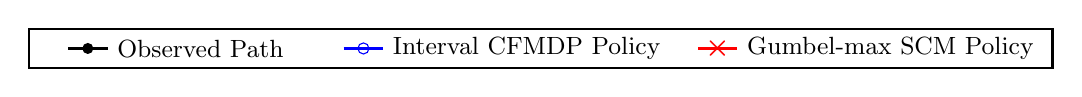
\begin{tikzpicture}[scale=1.0, every node/.style={scale=1.0}]
            \draw[thick, black] (-3, -0.25) rectangle (10, 0.25);
            %
            \draw[black, line width=1pt] (-2.5, 0.0) -- (-2,0.0);
            \fill[black] (-2.25,0.0) circle (2pt); %
            \node[right] at (-2,0.0) {\small Observed Path};
            
            %
            \draw[blue, line width=1pt] (1.0,0.0) -- (1.5,0.0);
            \node[draw=blue, circle, minimum size=4pt, inner sep=0pt] at (1.25,0.0) {}; %
            \node[right] at (1.5,0.0) {\small Interval CFMDP Policy};
            
            %
            \draw[red, line width=1pt] (5.5,0) -- (6,0);
            \node[red] at (5.75,0) {$\boldsymbol{\times}$}; %
            \node[right] at (6,0) {\small Gumbel-max SCM Policy};
        \end{tikzpicture}
    }\\
    %
    \subfigure[\footnotesize Lowest cumulative reward: Interval CFMDP ($312$), Gumbel-max SCM ($312$)]{%
        \resizebox{0.76\columnwidth}{!}{
             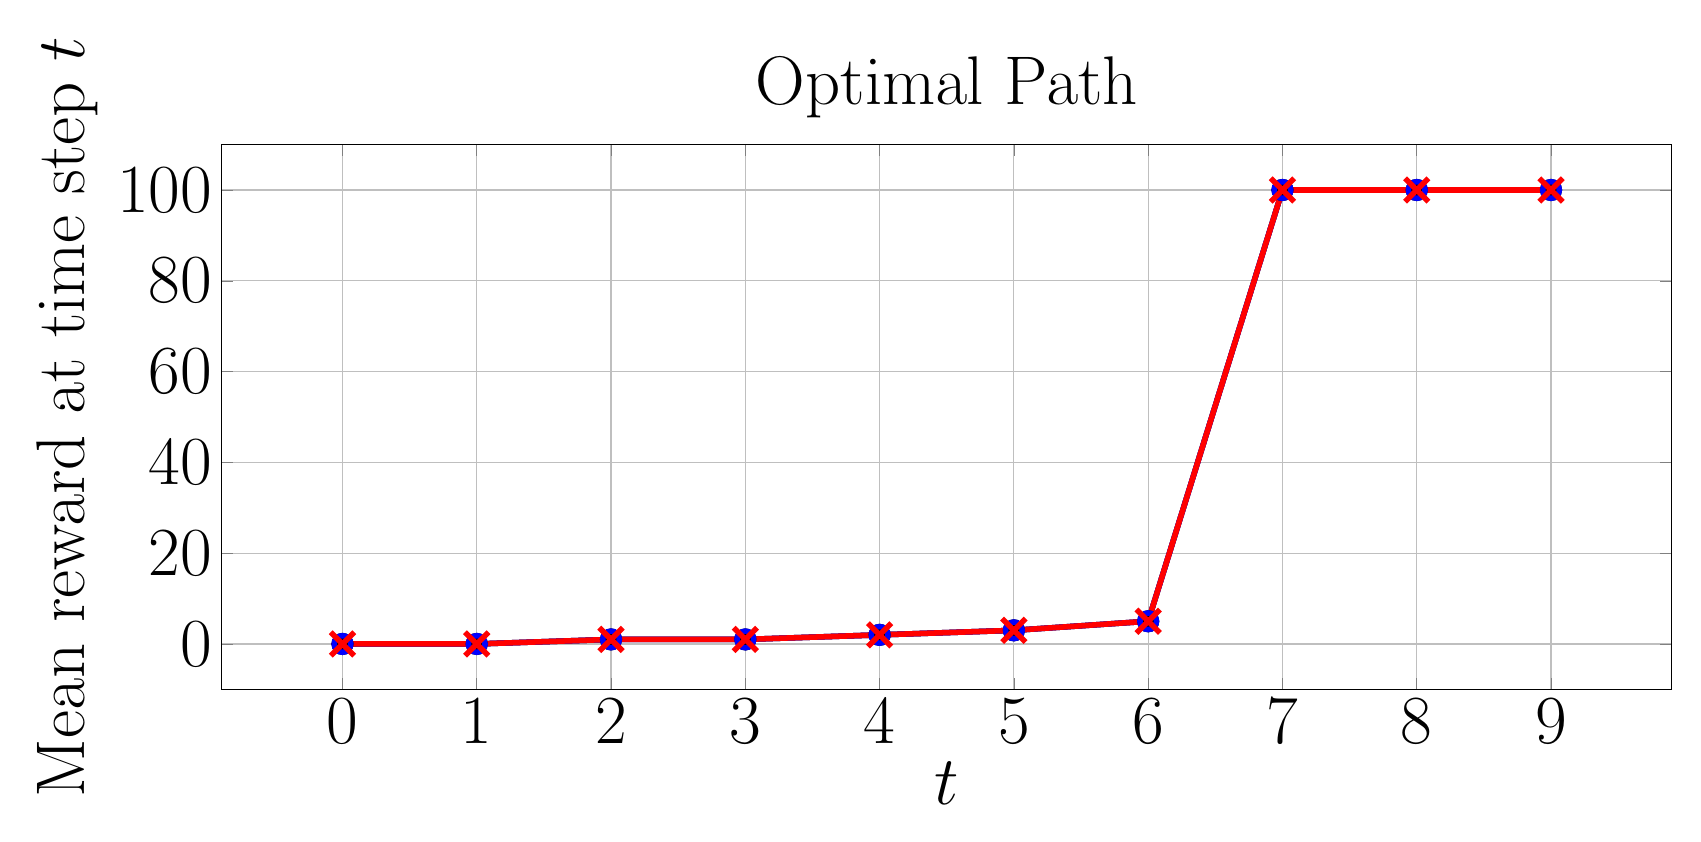
\begin{tikzpicture}
                \begin{axis}[
                    xlabel={$t$},
                    ylabel={Mean reward at time step $t$},
                    title={Optimal Path},
                    grid=both,
                    width=20cm, height=8.5cm,
                    every axis/.style={font=\Huge},
                    %
                ]
                \addplot[
                    color=black, %
                    mark=*, %
                    line width=2pt,
                    mark size=3pt,
                    error bars/.cd,
                    y dir=both, %
                    y explicit, %
                    error bar style={line width=1pt,solid},
                    error mark options={line width=1pt,mark size=4pt,rotate=90}
                ]
                coordinates {
                    (0, 0.0)  +- (0, 0.0)
                    (1, 0.0)  +- (0, 0.0) 
                    (2, 1.0)  +- (0, 0.0) 
                    (3, 1.0)  +- (0, 0.0)
                    (4, 2.0)  +- (0, 0.0)
                    (5, 3.0) +- (0, 0.0)
                    (6, 5.0) +- (0, 0.0)
                    (7, 100.0) +- (0, 0.0)
                    (8, 100.0) +- (0, 0.0)
                    (9, 100.0) +- (0, 0.0)
                };
                %
                \addplot[
                    color=blue, %
                    mark=o, %
                    line width=2pt,
                    mark size=3pt,
                    error bars/.cd,
                    y dir=both, %
                    y explicit, %
                    error bar style={line width=1pt,solid},
                    error mark options={line width=1pt,mark size=4pt,rotate=90}
                ]
                 coordinates {
                    (0, 0.0)  +- (0, 0.0)
                    (1, 0.0)  +- (0, 0.0) 
                    (2, 1.0)  +- (0, 0.0) 
                    (3, 1.0)  +- (0, 0.0)
                    (4, 2.0)  +- (0, 0.0)
                    (5, 3.0) +- (0, 0.0)
                    (6, 5.0) +- (0, 0.0)
                    (7, 100.0) +- (0, 0.0)
                    (8, 100.0) +- (0, 0.0)
                    (9, 100.0) +- (0, 0.0)
                };
                %
                \addplot[
                    color=red, %
                    mark=x, %
                    line width=2pt,
                    mark size=6pt,
                    error bars/.cd,
                    y dir=both, %
                    y explicit, %
                    error bar style={line width=1pt,solid},
                    error mark options={line width=1pt,mark size=4pt,rotate=90}
                ]
                coordinates {
                    (0, 0.0)  +- (0, 0.0)
                    (1, 0.0)  +- (0, 0.0) 
                    (2, 1.0)  +- (0, 0.0) 
                    (3, 1.0)  +- (0, 0.0)
                    (4, 2.0)  +- (0, 0.0)
                    (5, 3.0) +- (0, 0.0)
                    (6, 5.0) +- (0, 0.0)
                    (7, 100.0) +- (0, 0.0)
                    (8, 100.0) +- (0, 0.0)
                    (9, 100.0) +- (0, 0.0)
                };
                \end{axis}
            \end{tikzpicture}
         }
    }
    \hspace{1cm}
    \subfigure[\footnotesize Lowest cumulative reward: Interval CFMDP ($19$), Gumbel-max SCM ($-88$)]{%
         \resizebox{0.76\columnwidth}{!}{
            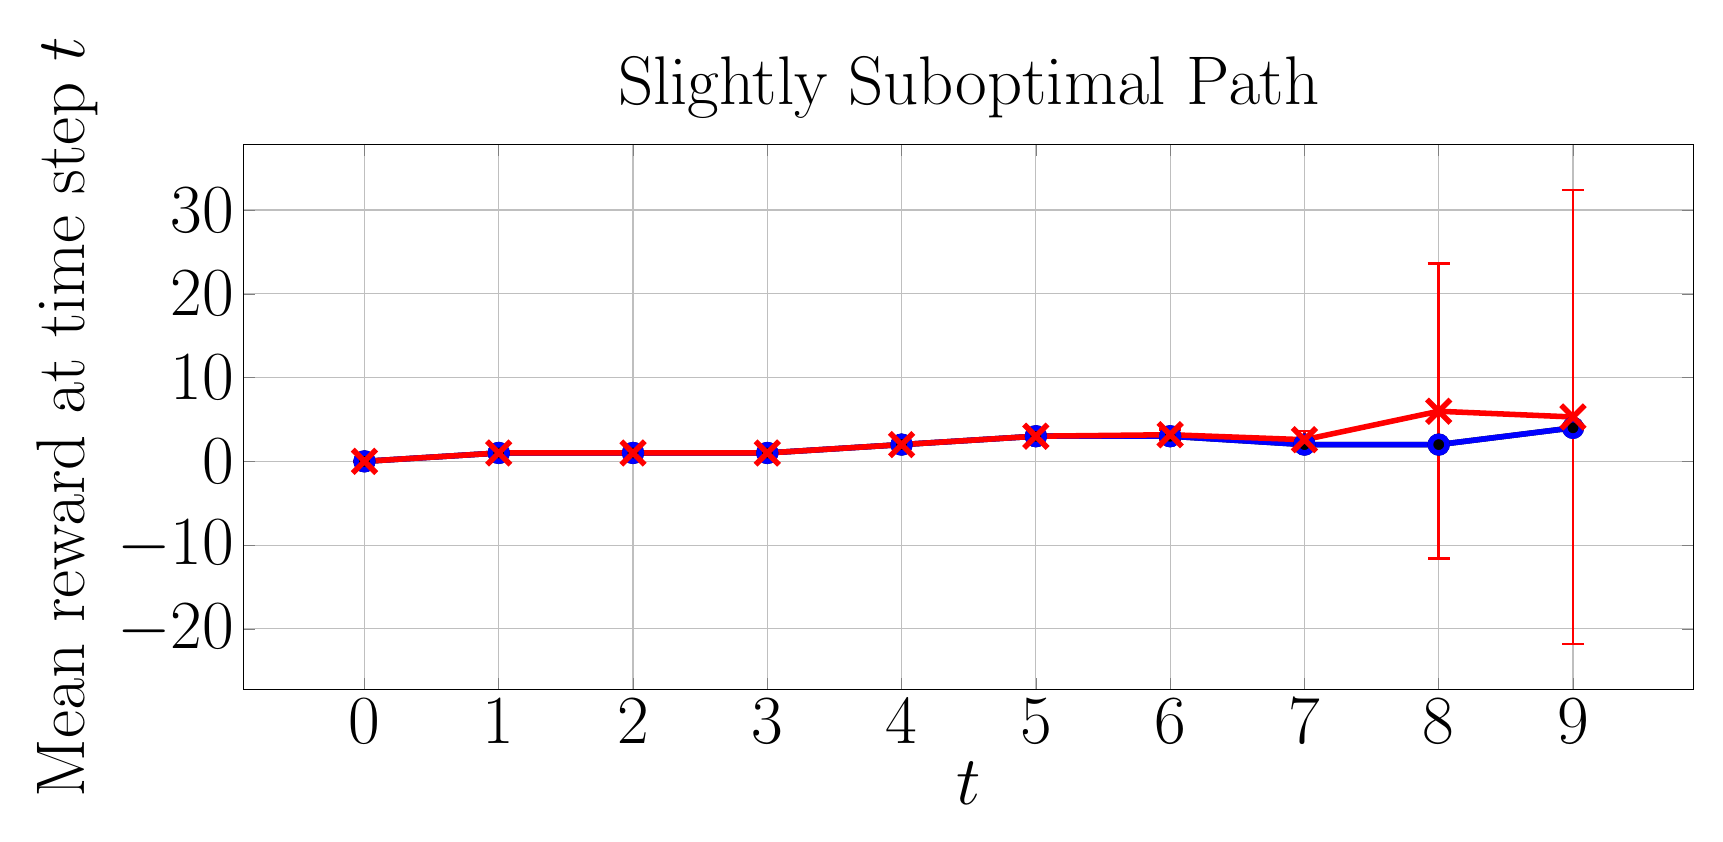
\begin{tikzpicture}
                \begin{axis}[
                    xlabel={$t$},
                    ylabel={Mean reward at time step $t$},
                    title={Slightly Suboptimal Path},
                    grid=both,
                    width=20cm, height=8.5cm,
                    every axis/.style={font=\Huge},
                    %
                ]
                \addplot[
                    color=black, %
                    mark=*, %
                    line width=2pt,
                    mark size=3pt,
                    error bars/.cd,
                    y dir=both, %
                    y explicit, %
                    error bar style={line width=1pt,solid},
                    error mark options={line width=1pt,mark size=4pt,rotate=90}
                ]
              coordinates {
                    (0, 0.0)  +- (0, 0.0)
                    (1, 1.0)  +- (0, 0.0) 
                    (2, 1.0)  +- (0, 0.0) 
                    (3, 1.0)  +- (0, 0.0)
                    (4, 2.0)  +- (0, 0.0)
                    (5, 3.0) +- (0, 0.0)
                    (6, 3.0) +- (0, 0.0)
                    (7, 2.0) +- (0, 0.0)
                    (8, 2.0) +- (0, 0.0)
                    (9, 4.0) +- (0, 0.0)
                };
                %
                \addplot[
                    color=blue, %
                    mark=o, %
                    line width=2pt,
                    mark size=3pt,
                    error bars/.cd,
                    y dir=both, %
                    y explicit, %
                    error bar style={line width=1pt,solid},
                    error mark options={line width=1pt,mark size=4pt,rotate=90}
                ]
              coordinates {
                    (0, 0.0)  +- (0, 0.0)
                    (1, 1.0)  +- (0, 0.0) 
                    (2, 1.0)  +- (0, 0.0) 
                    (3, 1.0)  +- (0, 0.0)
                    (4, 2.0)  +- (0, 0.0)
                    (5, 3.0) +- (0, 0.0)
                    (6, 3.0) +- (0, 0.0)
                    (7, 2.0) +- (0, 0.0)
                    (8, 2.0) +- (0, 0.0)
                    (9, 4.0) +- (0, 0.0)
                };
                %
                \addplot[
                    color=red, %
                    mark=x, %
                    line width=2pt,
                    mark size=6pt,
                    error bars/.cd,
                    y dir=both, %
                    y explicit, %
                    error bar style={line width=1pt,solid},
                    error mark options={line width=1pt,mark size=4pt,rotate=90}
                ]
                coordinates {
                    (0, 0.0)  +- (0, 0.0)
                    (1, 1.0)  +- (0, 0.0) 
                    (2, 1.0)  +- (0, 0.0) 
                    (3, 1.0)  +- (0, 0.0)
                    (4, 2.0)  += (0, 0.0)
                    (5, 3.0)  += (0, 0.0)
                    (6, 3.17847) += (0, 0.62606746) -= (0, 0.62606746)
                    (7, 2.5832885) += (0, 1.04598233) -= (0, 1.04598233)
                    (8, 5.978909) += (0, 17.60137623) -= (0, 17.60137623)
                    (9, 5.297059) += (0, 27.09227512) -= (0, 27.09227512)
                };
                \end{axis}
            \end{tikzpicture}
         }
    }\\[-1.5pt]
    \subfigure[\footnotesize Lowest cumulative reward: Interval CFMDP ($14$), Gumbel-max SCM ($-598$)]{%
         \resizebox{0.76\columnwidth}{!}{
             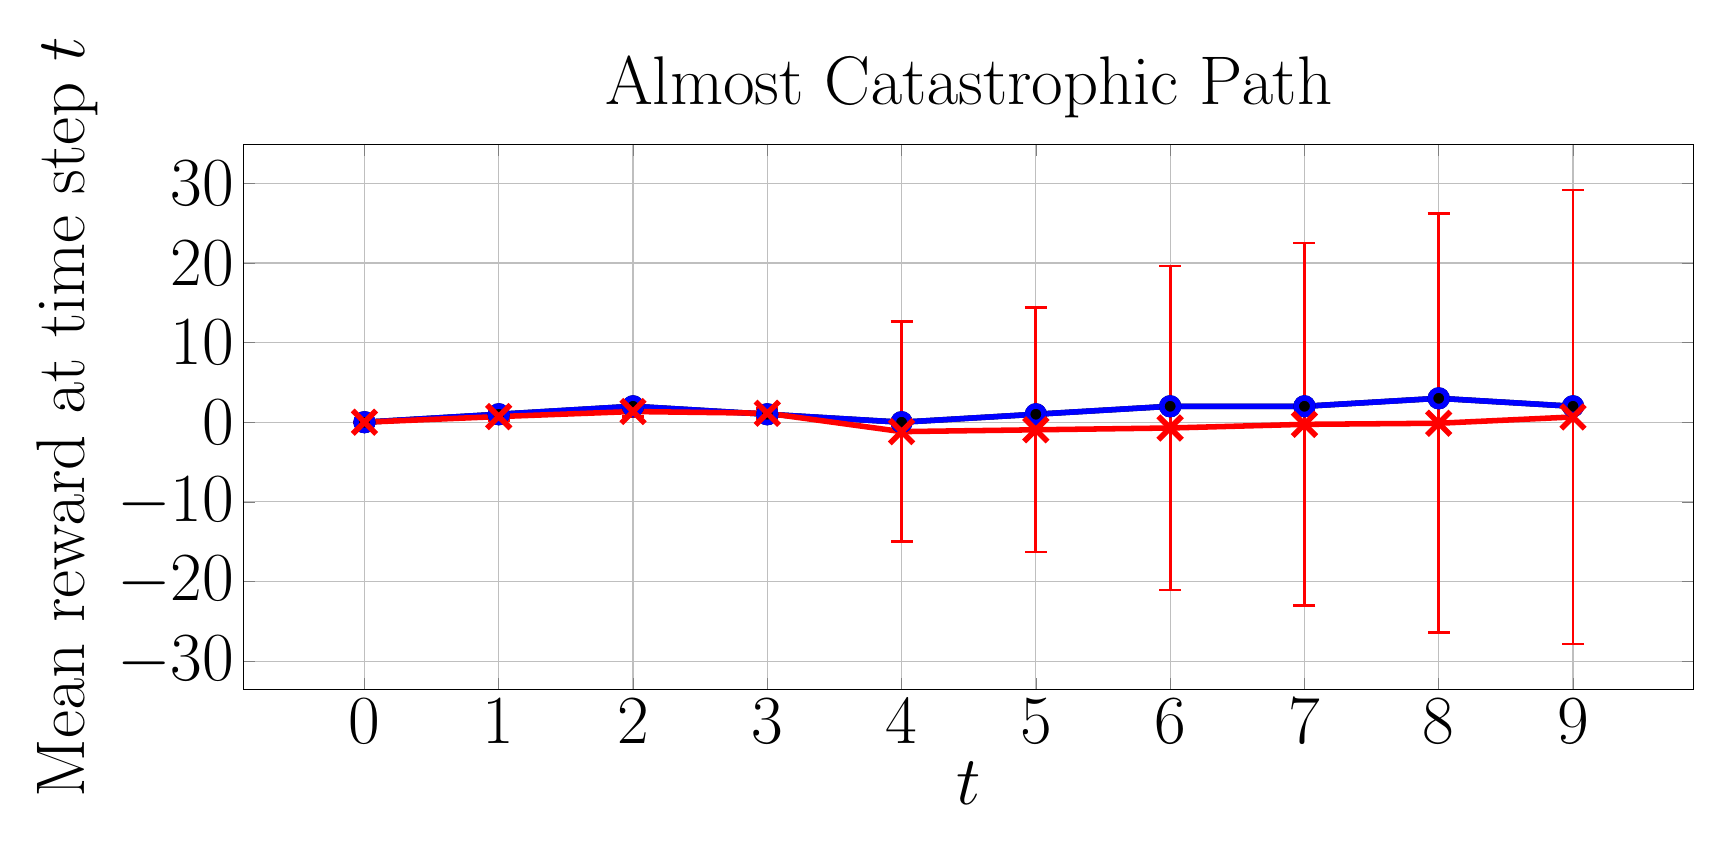
\begin{tikzpicture}
                \begin{axis}[
                    xlabel={$t$},
                    ylabel={Mean reward at time step $t$},
                    title={Almost Catastrophic Path},
                    grid=both,
                    width=20cm, height=8.5cm,
                    every axis/.style={font=\Huge},
                    %
                ]
                \addplot[
                    color=black, %
                    mark=*, %
                    line width=2pt,
                    mark size=3pt,
                    error bars/.cd,
                    y dir=both, %
                    y explicit, %
                    error bar style={line width=1pt,solid},
                    error mark options={line width=1pt,mark size=4pt,rotate=90}
                ]
                coordinates {
                    (0, 0.0)  +- (0, 0.0)
                    (1, 1.0)  +- (0, 0.0) 
                    (2, 2.0)  +- (0, 0.0) 
                    (3, 1.0)  +- (0, 0.0)
                    (4, 0.0)  +- (0, 0.0)
                    (5, 1.0) +- (0, 0.0)
                    (6, 2.0) +- (0, 0.0)
                    (7, 2.0) +- (0, 0.0)
                    (8, 3.0) +- (0, 0.0)
                    (9, 2.0) +- (0, 0.0)
                };
                %
                \addplot[
                    color=blue, %
                    mark=o, %
                    line width=2pt,
                    mark size=3pt,
                    error bars/.cd,
                    y dir=both, %
                    y explicit, %
                    error bar style={line width=1pt,solid},
                    error mark options={line width=1pt,mark size=4pt,rotate=90}
                ]
                coordinates {
                    (0, 0.0)  +- (0, 0.0)
                    (1, 1.0)  +- (0, 0.0) 
                    (2, 2.0)  +- (0, 0.0) 
                    (3, 1.0)  +- (0, 0.0)
                    (4, 0.0)  +- (0, 0.0)
                    (5, 1.0) +- (0, 0.0)
                    (6, 2.0) +- (0, 0.0)
                    (7, 2.0) +- (0, 0.0)
                    (8, 3.0) +- (0, 0.0)
                    (9, 2.0) +- (0, 0.0)
                };
                %
                \addplot[
                    color=red, %
                    mark=x, %
                    line width=2pt,
                    mark size=6pt,
                    error bars/.cd,
                    y dir=both, %
                    y explicit, %
                    error bar style={line width=1pt,solid},
                    error mark options={line width=1pt,mark size=4pt,rotate=90}
                ]
                coordinates {
                    (0, 0.0)  +- (0, 0.0)
                    (1, 0.7065655)  +- (0, 0.4553358) 
                    (2, 1.341673)  +- (0, 0.67091621) 
                    (3, 1.122926)  +- (0, 0.61281824)
                    (4, -1.1821935)  +- (0, 13.82444042)
                    (5, -0.952399)  +- (0, 15.35195457)
                    (6, -0.72672) +- (0, 20.33508414)
                    (7, -0.268983) +- (0, 22.77861454)
                    (8, -0.1310835) +- (0, 26.31013314)
                    (9, 0.65806) +- (0, 28.50670214)
                };
                %
            %
            %
            %
            %
            %
            %
            %
            %
            %
            %
            %
            %
            %
            %
            %
            %
            %
            %
                \end{axis}
            \end{tikzpicture}
         }
    }
    \hspace{1cm}
    \subfigure[\footnotesize Lowest cumulative reward: Interval CFMDP ($-698$), Gumbel-max SCM ($-698$)]{%
         \resizebox{0.76\columnwidth}{!}{
            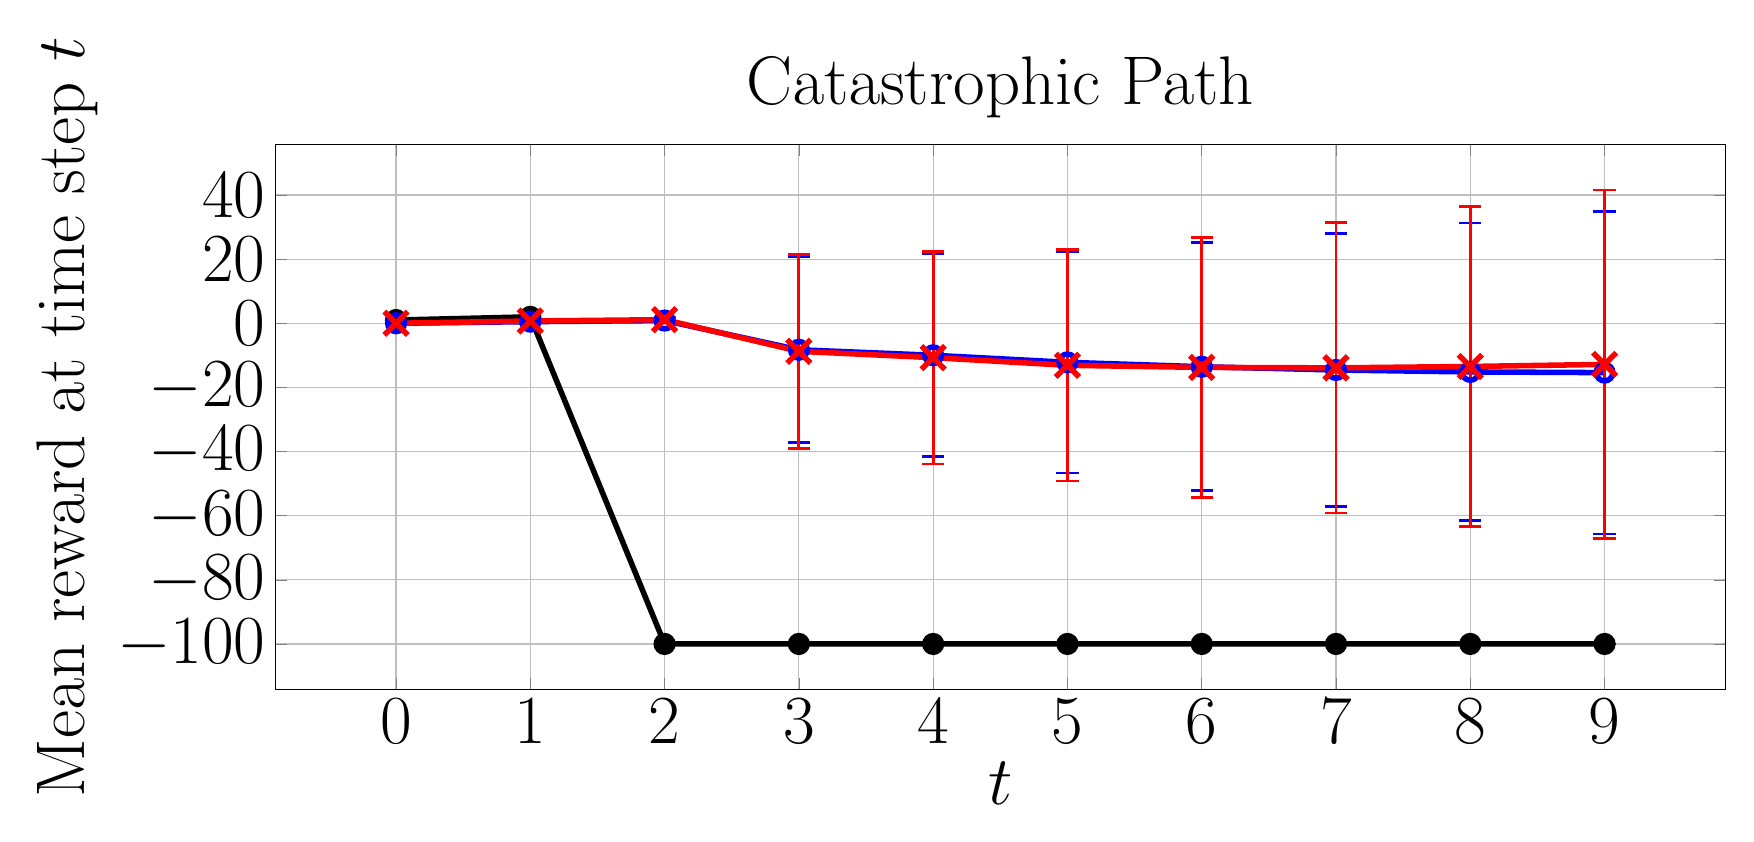
\begin{tikzpicture}
                \begin{axis}[
                    xlabel={$t$},
                    ylabel={Mean reward at time step $t$},
                    title={Catastrophic Path},
                    grid=both,
                    width=20cm, height=8.5cm,
                    every axis/.style={font=\Huge},
                    %
                ]
                \addplot[
                    color=black, %
                    mark=*, %
                    line width=2pt,
                    mark size=3pt,
                    error bars/.cd,
                    y dir=both, %
                    y explicit, %
                    error bar style={line width=1pt,solid},
                    error mark options={line width=1pt,mark size=4pt,rotate=90}
                ]
                coordinates {
                    (0, 1.0)  +- (0, 0.0)
                    (1, 2.0)  +- (0, 0.0) 
                    (2, -100.0)  +- (0, 0.0) 
                    (3, -100.0)  +- (0, 0.0)
                    (4, -100.0)  +- (0, 0.0)
                    (5, -100.0) +- (0, 0.0)
                    (6, -100.0) +- (0, 0.0)
                    (7, -100.0) +- (0, 0.0)
                    (8, -100.0) +- (0, 0.0)
                    (9, -100.0) +- (0, 0.0)
                };
                %
                \addplot[
                    color=blue, %
                    mark=o, %
                    line width=2pt,
                    mark size=3pt,
                    error bars/.cd,
                    y dir=both, %
                    y explicit, %
                    error bar style={line width=1pt,solid},
                    error mark options={line width=1pt,mark size=4pt,rotate=90}
                ]
                coordinates {
                    (0, 0.0)  +- (0, 0.0)
                    (1, 0.504814)  +- (0, 0.49997682) 
                    (2, 0.8439835)  +- (0, 0.76831917) 
                    (3, -8.2709165)  +- (0, 28.93656754)
                    (4, -9.981082)  +- (0, 31.66825363)
                    (5, -12.1776325) +- (0, 34.53463233)
                    (6, -13.556076) +- (0, 38.62845372)
                    (7, -14.574418) +- (0, 42.49603359)
                    (8, -15.1757075) +- (0, 46.41913968)
                    (9, -15.3900395) +- (0, 50.33563368)
                };
                %
                \addplot[
                    color=red, %
                    mark=x, %
                    line width=2pt,
                    mark size=6pt,
                    error bars/.cd,
                    y dir=both, %
                    y explicit, %
                    error bar style={line width=1pt,solid},
                    error mark options={line width=1pt,mark size=4pt,rotate=90}
                ]
                coordinates {
                    (0, 0.0)  +- (0, 0.0)
                    (1, 0.701873)  +- (0, 0.45743556) 
                    (2, 1.1227805)  +- (0, 0.73433129) 
                    (3, -8.7503255)  +- (0, 30.30257976)
                    (4, -10.722092)  +- (0, 33.17618589)
                    (5, -13.10721)  +- (0, 36.0648089)
                    (6, -13.7631645) +- (0, 40.56553451)
                    (7, -13.909043) +- (0, 45.23829402)
                    (8, -13.472517) +- (0, 49.96270296)
                    (9, -12.8278835) +- (0, 54.38618735)
                };
                %
            %
            %
            %
            %
            %
            %
            %
            %
            %
            %
            %
            %
            %
            %
            %
            %
            %
            %
                \end{axis}
            \end{tikzpicture}
         }
    }
    \caption{Average instant reward of CF paths induced by policies on GridWorld $p=0.4$.}
    \label{fig: reward p=0.4}
\end{figure*}

\subsection{Experimental Setup}
To compare policy performance, we measure the average rewards of counterfactual paths induced by our policy and the Gumbel-max policy by uniformly sampling $200$ counterfactual MDPs from the ICFMDP and generating $10,000$ counterfactual paths over each sampled CFMDP. \jl{Since the interval CFMDP depends on the observed path, we select $4$  paths of varying optimality to evaluate how the observed path impacts the performance of both policies: an optimal path, a slightly suboptimal path that could reach the optimal reward with a few changes, a catastrophic path that enters a catastrophic, terminal state with low reward, and an almost catastrophic path that was close to entering a catastrophic state.} When measuring the average probability bound widths and execution time needed to generate the ICFMDPs, we averaged over $20$ randomly generated observed paths
\footnote{Further training details are provided in Appendix \ref{app: training details}, and the code is provided at \href{https://github.com/ddv-lab/robust-cf-inference-in-MDPs}{https://github.com/ddv-lab/robust-cf-inference-in-MDPs}
%
%
.}.

\subsection{GridWorld}
\jl{The GridWorld MDP is a $4 \times 4$ grid where an agent must navigate from the top-left corner to the goal state in the bottom-right corner, avoiding a dangerous terminal state in the centre. At each time step, the agent can move up, down, left, or right, but there is a small probability (controlled by hyper-parameter $p$) of moving in an unintended direction. As the agent nears the goal, the reward for each state increases, culminating in a reward of $+100$ for reaching the goal. Entering the dangerous state results in a penalty of $-100$. We use two versions of GridWorld: a less stochastic version with $p=0.9$ (i.e., $90$\% chance of moving in the chosen direction) and a more stochastic version with $p=0.4$.}

\paragraph{GridWorld ($p=0.9$)}
When $p=0.9$, the counterfactual probability bounds are typically narrow (see Table \ref{tab:nonzero_probs} for average measurements). Consequently, as shown in Figure \ref{fig: reward p=0.9}, both policies are nearly identical and perform similarly well across the optimal, slightly suboptimal, and catastrophic paths.
%
However, for the almost catastrophic path, the interval CFMDP path is more conservative and follows the observed path more closely (as this is where the probability bounds are narrowest), which typically requires one additional step to reach the goal state than the Gumbel-max SCM policy.
%

\paragraph{GridWorld ($p=0.4$)}
\jl{When $p=0.4$, the GridWorld environment becomes more uncertain, increasing the risk of entering the dangerous state even if correct actions are chosen. Thus, as shown in Figure \ref{fig: reward p=0.4}, the interval CFMDP policy adopts a more conservative approach, avoiding deviation from the observed policy if it cannot guarantee higher counterfactual rewards (see the slightly suboptimal and almost catastrophic paths), whereas the Gumbel-max SCM is inconsistent: it can yield higher rewards, but also much lower rewards, reflected in the wide error bars.} For the catastrophic path, both policies must deviate from the observed path to achieve a higher reward and, in this case, perform similarly.
%
%
%
%
\subsection{Sepsis}
The Sepsis MDP \citep{oberst2019counterfactual} simulates trajectories of Sepsis patients. Each state consists of four vital signs (heart rate, blood pressure, oxygen concentration, and glucose levels), categorised as low, normal, or high.
and three treatments that can be toggled on/off at each time step (8 actions in total). Unlike \citet{oberst2019counterfactual}, we scale rewards based on the number of out-of-range vital signs, between $-1000$ (patient dies) and $1000$ (patient discharged). \jl{Like the GridWorld $p=0.4$ experiment, the Sepsis MDP is highly uncertain, as many states are equally likely to lead to optimal and poor outcomes. Thus, as shown in Figure \ref{fig: reward sepsis}, both policies follow the observed optimal and almost catastrophic paths to guarantee rewards are no worse than the observation.} However, improving the catastrophic path requires deviating from the observation. Here, the Gumbel-max SCM policy, on average, performs better than the interval CFMDP policy. But, since both policies have lower bounds clipped at $-1000$, neither policy reliably improves over the observation. In contrast, for the slightly suboptimal path, the interval CFMDP policy performs significantly better, shown by its higher lower bounds. 
Moreover, in these two cases, the worst-case counterfactual path generated by the interval CFMDP policy is better than that of the Gumbel-max SCM policy,
indicating its greater robustness.
%
\begin{figure*}
    \centering
     \resizebox{0.6\textwidth}{!}{
        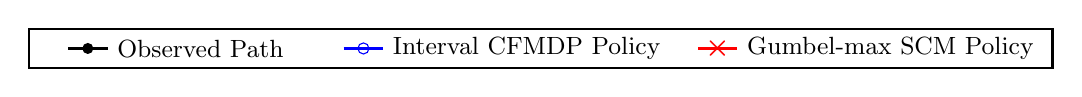
\begin{tikzpicture}[scale=1.0, every node/.style={scale=1.0}]
            \draw[thick, black] (-3, -0.25) rectangle (10, 0.25);
            %
            \draw[black, line width=1pt] (-2.5, 0.0) -- (-2,0.0);
            \fill[black] (-2.25,0.0) circle (2pt); %
            \node[right] at (-2,0.0) {\small Observed Path};
            
            %
            \draw[blue, line width=1pt] (1.0,0.0) -- (1.5,0.0);
            \node[draw=blue, circle, minimum size=4pt, inner sep=0pt] at (1.25,0.0) {}; %
            \node[right] at (1.5,0.0) {\small Interval CFMDP Policy};
            
            %
            \draw[red, line width=1pt] (5.5,0) -- (6,0);
            \node[red] at (5.75,0) {$\boldsymbol{\times}$}; %
            \node[right] at (6,0) {\small Gumbel-max SCM Policy};
        \end{tikzpicture}
    }\\
    \subfigure[\footnotesize Lowest cumulative reward: Interval CFMDP ($8000$), Gumbel-max SCM ($8000$)]{%
         \resizebox{0.76\columnwidth}{!}{
             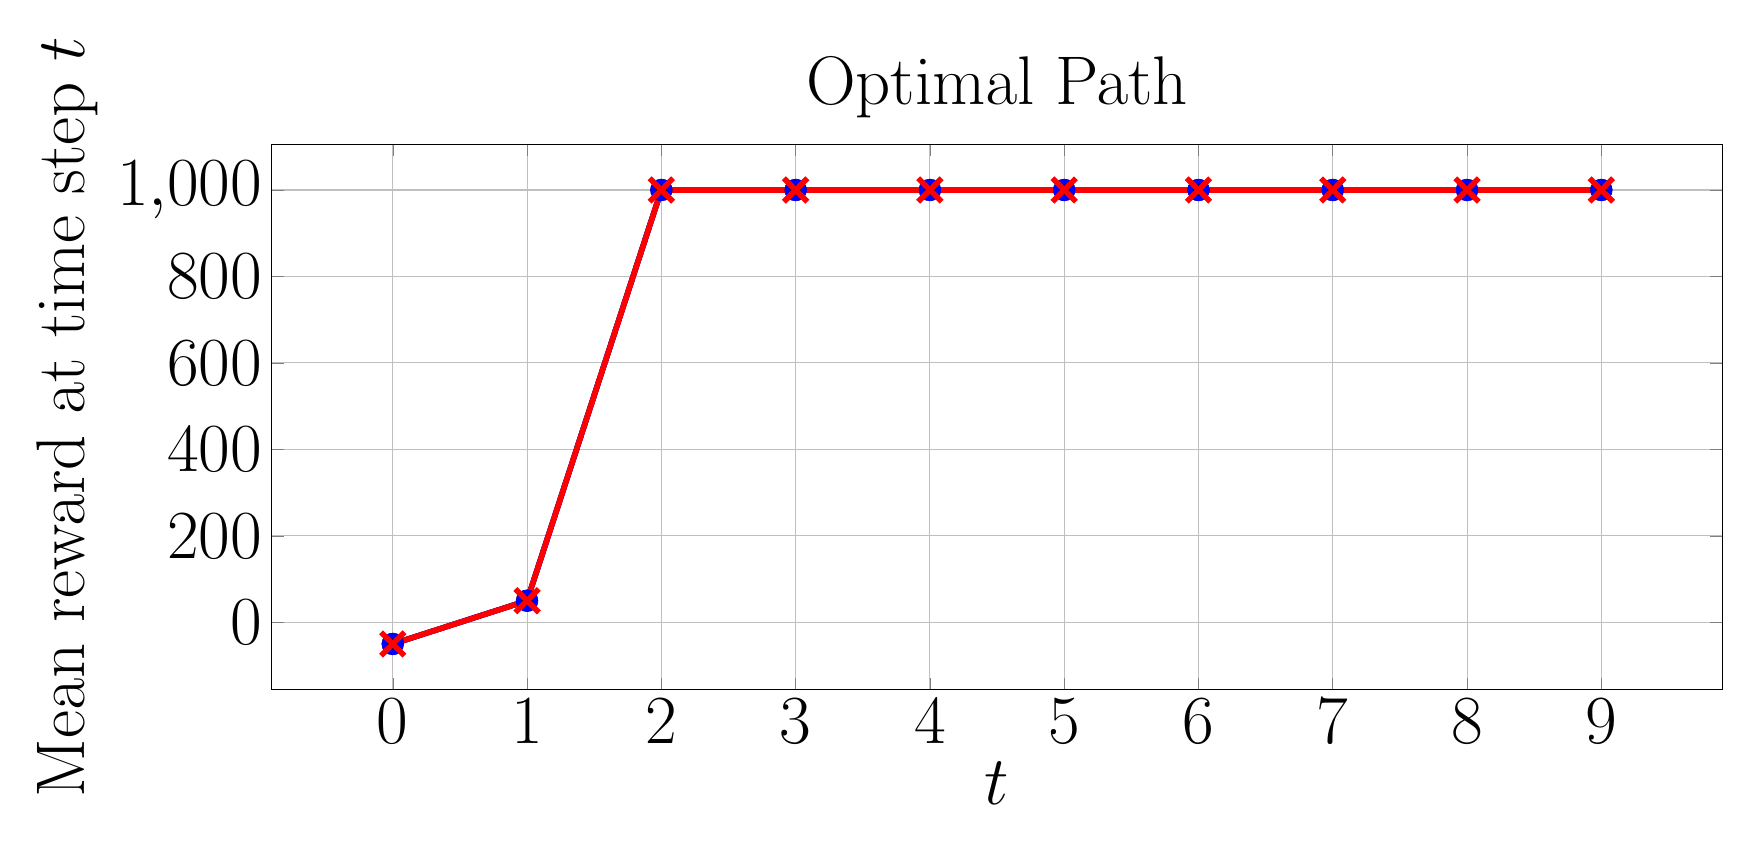
\begin{tikzpicture}
                \begin{axis}[
                    xlabel={$t$},
                    ylabel={Mean reward at time step $t$},
                    title={Optimal Path},
                    grid=both,
                    width=20cm, height=8.5cm,
                    every axis/.style={font=\Huge},
                    %
                ]
                \addplot[
                    color=black, %
                    mark=*, %
                    line width=2pt,
                    mark size=3pt,
                ]
                coordinates {
                    (0, -50.0)
                    (1, 50.0)
                    (2, 1000.0)
                    (3, 1000.0)
                    (4, 1000.0)
                    (5, 1000.0)
                    (6, 1000.0)
                    (7, 1000.0)
                    (8, 1000.0)
                    (9, 1000.0)
                };
                %
                \addplot[
                    color=blue, %
                    mark=o, %
                    line width=2pt,
                    mark size=3pt,
                    error bars/.cd,
                    y dir=both, %
                    y explicit, %
                    error bar style={line width=1pt,solid},
                    error mark options={line width=1pt,mark size=4pt,rotate=90}
                ]
                coordinates {
                    (0, -50.0)  +- (0, 0.0)
                    (1, 50.0)  +- (0, 0.0) 
                    (2, 1000.0)  +- (0, 0.0) 
                    (3, 1000.0)  +- (0, 0.0)
                    (4, 1000.0)  +- (0, 0.0)
                    (5, 1000.0) +- (0, 0.0)
                    (6, 1000.0) +- (0, 0.0)
                    (7, 1000.0) +- (0, 0.0)
                    (8, 1000.0) +- (0, 0.0)
                    (9, 1000.0) +- (0, 0.0)
                };
                %
                \addplot[
                    color=red, %
                    mark=x, %
                    line width=2pt,
                    mark size=6pt,
                    error bars/.cd,
                    y dir=both, %
                    y explicit, %
                    error bar style={line width=1pt,solid},
                    error mark options={line width=1pt,mark size=4pt,rotate=90}
                ]
                coordinates {
                    (0, -50.0)  +- (0, 0.0)
                    (1, 50.0)  +- (0, 0.0) 
                    (2, 1000.0)  +- (0, 0.0) 
                    (3, 1000.0)  +- (0, 0.0)
                    (4, 1000.0)  +- (0, 0.0)
                    (5, 1000.0) +- (0, 0.0)
                    (6, 1000.0) +- (0, 0.0)
                    (7, 1000.0) +- (0, 0.0)
                    (8, 1000.0) +- (0, 0.0)
                    (9, 1000.0) +- (0, 0.0)
                };
                %
                \end{axis}
            \end{tikzpicture}
         }
    }
    \hspace{1cm}
    \subfigure[\footnotesize Lowest cumulative reward: Interval CFMDP ($-5980$), Gumbel-max SCM ($-8000$)]{%
         \resizebox{0.76\columnwidth}{!}{
            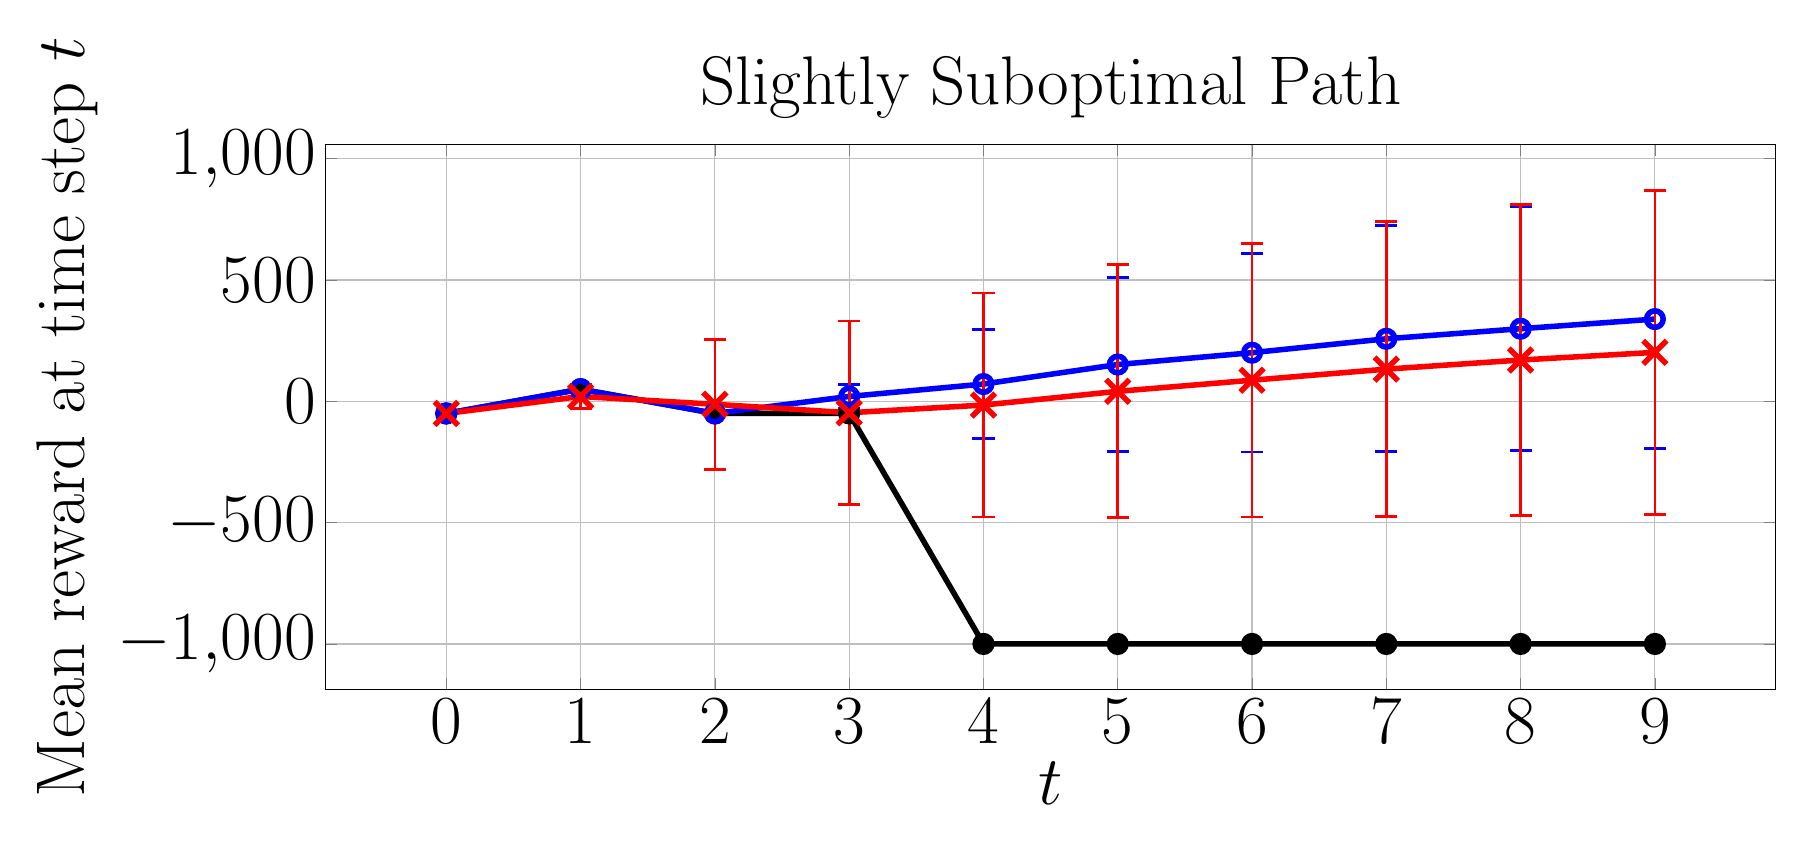
\begin{tikzpicture}
                \begin{axis}[
                    xlabel={$t$},
                    ylabel={Mean reward at time step $t$},
                    title={Slightly Suboptimal Path},
                    grid=both,
                    width=20cm, height=8.5cm,
                    every axis/.style={font=\Huge},
                    %
                ]
               \addplot[
                    color=black, %
                    mark=*, %
                    line width=2pt,
                    mark size=3pt,
                ]
                coordinates {
                    (0, -50.0)
                    (1, 50.0)
                    (2, -50.0)
                    (3, -50.0)
                    (4, -1000.0)
                    (5, -1000.0)
                    (6, -1000.0)
                    (7, -1000.0)
                    (8, -1000.0)
                    (9, -1000.0)
                };
                %
                \addplot[
                    color=blue, %
                    mark=o, %
                    line width=2pt,
                    mark size=3pt,
                    error bars/.cd,
                    y dir=both, %
                    y explicit, %
                    error bar style={line width=1pt,solid},
                    error mark options={line width=1pt,mark size=4pt,rotate=90}
                ]
                coordinates {
                    (0, -50.0)  +- (0, 0.0)
                    (1, 50.0)  +- (0, 0.0) 
                    (2, -50.0)  +- (0, 0.0) 
                    (3, 20.0631)  +- (0, 49.97539413)
                    (4, 71.206585)  +- (0, 226.02033693)
                    (5, 151.60797) +- (0, 359.23292559)
                    (6, 200.40593) +- (0, 408.86185176)
                    (7, 257.77948) +- (0, 466.10372804)
                    (8, 299.237465) +- (0, 501.82579506)
                    (9, 338.9129) +- (0, 532.06124996)
                };
                %
                \addplot[
                    color=red, %
                    mark=x, %
                    line width=2pt,
                    mark size=6pt,
                    error bars/.cd,
                    y dir=both, %
                    y explicit, %
                    error bar style={line width=1pt,solid},
                    error mark options={line width=1pt,mark size=4pt,rotate=90}
                ]
                coordinates {
                    (0, -50.0)  +- (0, 0.0)
                    (1, 20.00736)  +- (0, 49.99786741) 
                    (2, -12.282865)  +- (0, 267.598755) 
                    (3, -47.125995)  +- (0, 378.41755832)
                    (4, -15.381965)  +- (0, 461.77616558)
                    (5, 41.15459) +- (0, 521.53189262)
                    (6, 87.01595) +- (0, 564.22243126 )
                    (7, 132.62376) +- (0, 607.31338037)
                    (8, 170.168145) +- (0, 641.48013693)
                    (9, 201.813135) +- (0, 667.29441777)
                };
                %
                %
                %
                %
                %
                %
                %
                %
                %
                %
                %
                %
                %
                %
                %
                %
                %
                %
                %
                \end{axis}
            \end{tikzpicture}
         }
    }\\[-1.5pt]
    \subfigure[\footnotesize Lowest cumulative reward: Interval CFMDP ($100$), Gumbel-max SCM ($100$)]{%
         \resizebox{0.76\columnwidth}{!}{
             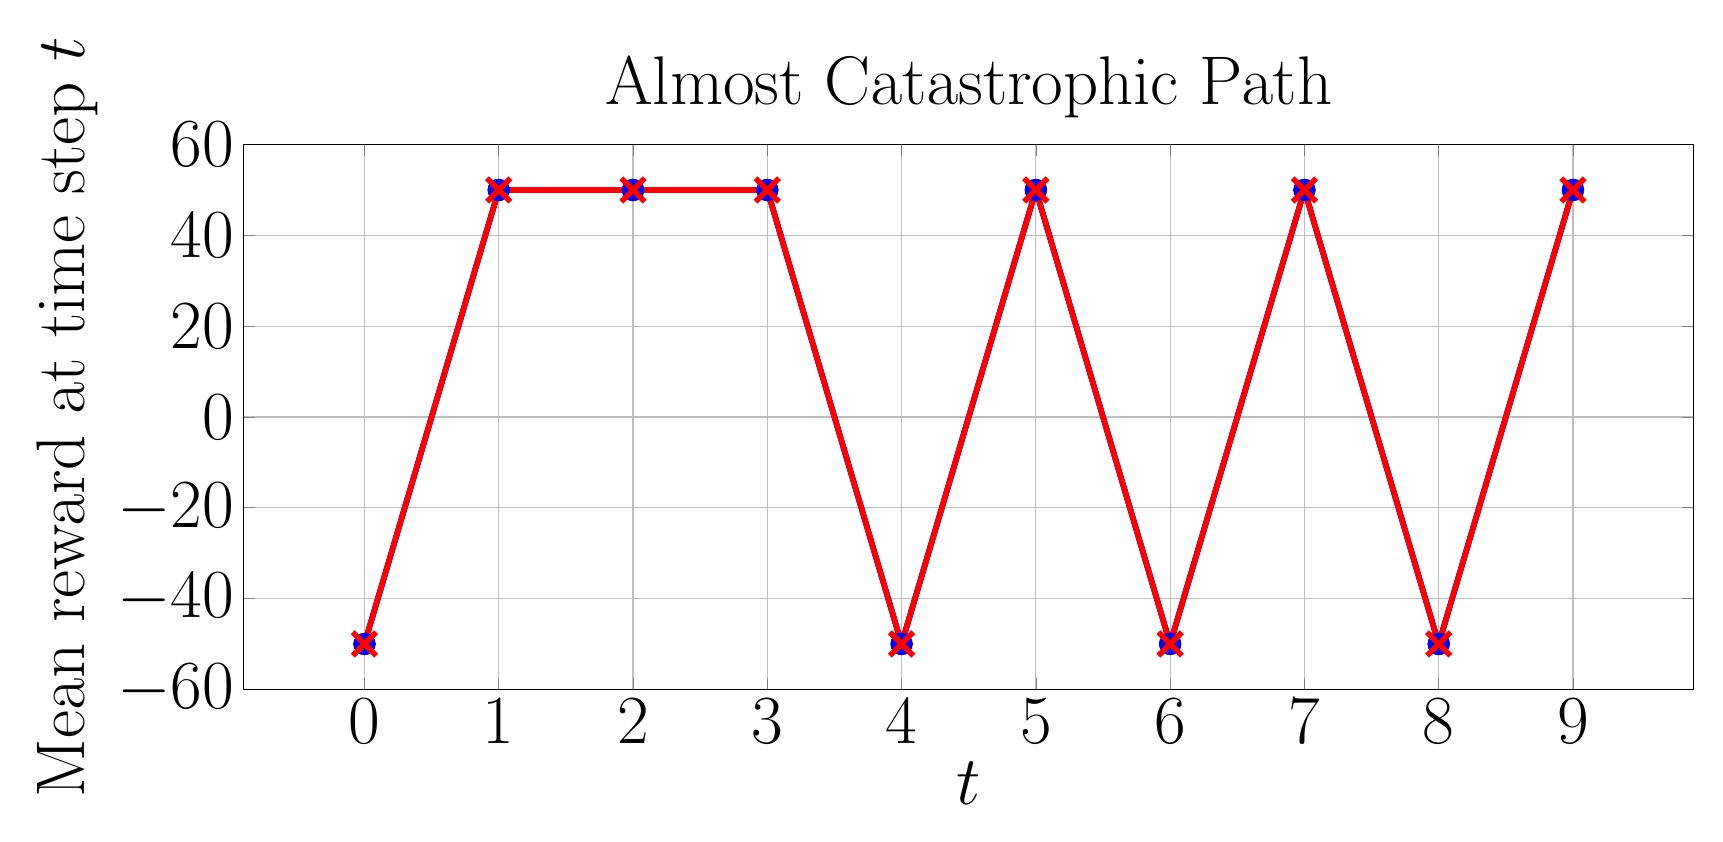
\begin{tikzpicture}
                \begin{axis}[
                    xlabel={$t$},
                    ylabel={Mean reward at time step $t$},
                    title={Almost Catastrophic Path},
                    grid=both,
                    every axis/.style={font=\Huge},
                    width=20cm, height=8.5cm,
                    %
                ]
               \addplot[
                    color=black, %
                    mark=*, %
                    line width=2pt,
                    mark size=3pt,
                ]
                coordinates {
                    (0, -50.0)
                    (1, 50.0)
                    (2, 50.0)
                    (3, 50.0)
                    (4, -50.0)
                    (5, 50.0)
                    (6, -50.0)
                    (7, 50.0)
                    (8, -50.0)
                    (9, 50.0)
                };
                %
                %
                \addplot[
                    color=blue, %
                    mark=o, %
                    line width=2pt,
                    mark size=3pt,
                    error bars/.cd,
                    y dir=both, %
                    y explicit, %
                    error bar style={line width=1pt,solid},
                    error mark options={line width=1pt,mark size=4pt,rotate=90}
                ]
                coordinates {
                    (0, -50.0)  +- (0, 0.0)
                    (1, 50.0)  +- (0, 0.0) 
                    (2, 50.0)  +- (0, 0.0) 
                    (3, 50.0)  +- (0, 0.0)
                    (4, -50.0)  +- (0, 0.0)
                    (5, 50.0) +- (0, 0.0)
                    (6, -50.0) +- (0, 0.0)
                    (7, 50.0) +- (0, 0.0)
                    (8, -50.0) +- (0, 0.0)
                    (9, 50.0) +- (0, 0.0)
                };
                %
                \addplot[
                    color=red, %
                    mark=x, %
                    line width=2pt,
                    mark size=6pt,
                    error bars/.cd,
                    y dir=both, %
                    y explicit, %
                    error bar style={line width=1pt,solid},
                    error mark options={line width=1pt,mark size=4pt,rotate=90}
                ]
                coordinates {
                    (0, -50.0)  +- (0, 0.0)
                    (1, 50.0)  +- (0, 0.0) 
                    (2, 50.0)  +- (0, 0.0) 
                    (3, 50.0)  +- (0, 0.0)
                    (4, -50.0)  +- (0, 0.0)
                    (5, 50.0) +- (0, 0.0)
                    (6, -50.0) +- (0, 0.0)
                    (7, 50.0) +- (0, 0.0)
                    (8, -50.0) +- (0, 0.0)
                    (9, 50.0) +- (0, 0.0)
                };
                %
                %
                %
                %
                %
                %
                %
                %
                %
                %
                %
                %
                %
                %
                %
                %
                %
                %
                %
                \end{axis}
            \end{tikzpicture}
         }
    }
    \hspace{1cm}
    \subfigure[\footnotesize Lowest cumulative reward: Interval CFMDP ($-7150$), Gumbel-max SCM ($-9050$)]{%
         \resizebox{0.76\columnwidth}{!}{
            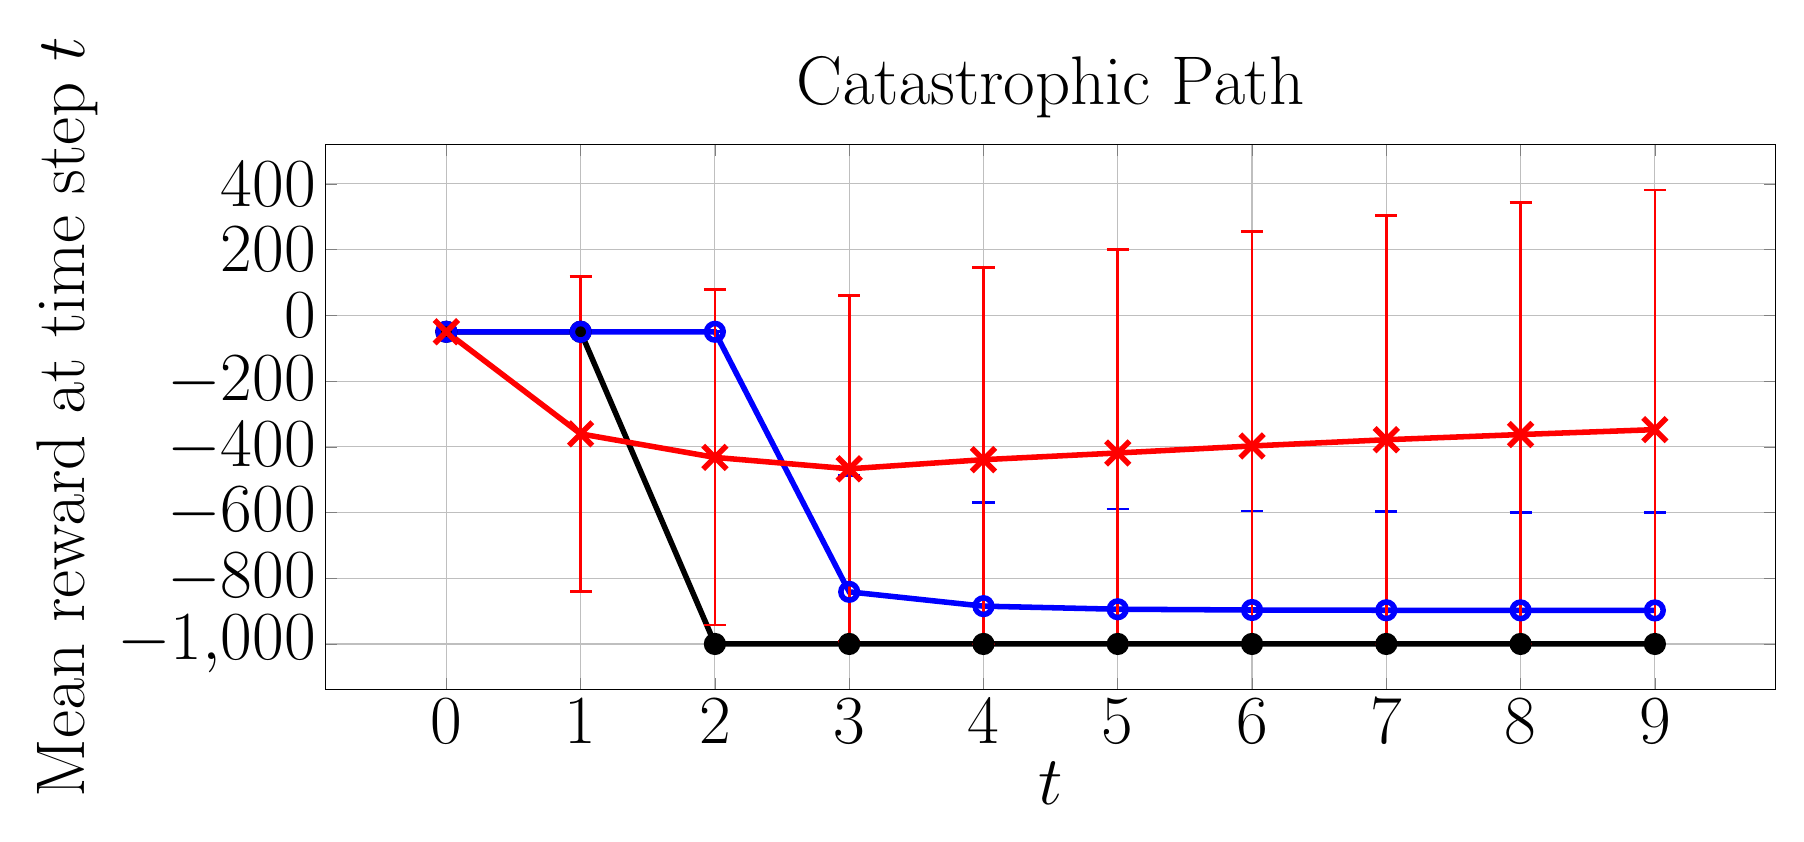
\begin{tikzpicture}
                \begin{axis}[
                    xlabel={$t$},
                    ylabel={Mean reward at time step $t$},
                    title={Catastrophic Path},
                    grid=both,
                    width=20cm, height=8.5cm,
                    every axis/.style={font=\Huge},
                    %
                ]
               \addplot[
                    color=black, %
                    mark=*, %
                    line width=2pt,
                    mark size=3pt,
                ]
                coordinates {
                    (0, -50.0)
                    (1, -50.0)
                    (2, -1000.0)
                    (3, -1000.0)
                    (4, -1000.0)
                    (5, -1000.0)
                    (6, -1000.0)
                    (7, -1000.0)
                    (8, -1000.0)
                    (9, -1000.0)
                };
                %
                %
                \addplot[
                    color=blue, %
                    mark=o, %
                    line width=2pt,
                    mark size=3pt,
                    error bars/.cd,
                    y dir=both, %
                    y explicit, %
                    error bar style={line width=1pt,solid},
                    error mark options={line width=1pt,mark size=4pt,rotate=90}
                ]
                coordinates {
                    (0, -50.0)  +- (0, 0.0)
                    (1, -50.0)  +- (0, 0.0) 
                    (2, -50.0)  +- (0, 0.0) 
                    (3, -841.440725)  += (0, 354.24605512) -= (0, 158.559275)
                    (4, -884.98225)  += (0, 315.37519669) -= (0, 115.01775)
                    (5, -894.330425) += (0, 304.88572805) -= (0, 105.669575)
                    (6, -896.696175) += (0, 301.19954514) -= (0, 103.303825)
                    (7, -897.4635) += (0, 299.61791279) -= (0, 102.5365)
                    (8, -897.77595) += (0, 298.80392585) -= (0, 102.22405)
                    (9, -897.942975) += (0, 298.32920557) -= (0, 102.057025)
                };
                %
                \addplot[
                    color=red, %
                    mark=x, %
                    line width=2pt,
                    mark size=6pt,
                    error bars/.cd,
                    y dir=both, %
                    y explicit, %
                    error bar style={line width=1pt,solid},
                    error mark options={line width=1pt,mark size=4pt,rotate=90}
                ]
            coordinates {
                    (0, -50.0)  +- (0, 0.0)
                    (1, -360.675265)  +- (0, 479.39812699) 
                    (2, -432.27629)  +- (0, 510.38620897) 
                    (3, -467.029545)  += (0, 526.36009628) -= (0, 526.36009628)
                    (4, -439.17429)  += (0, 583.96638919) -= (0, 560.82571)
                    (5, -418.82704) += (0, 618.43027478) -= (0, 581.17296)
                    (6, -397.464895) += (0, 652.67322574) -= (0, 602.535105)
                    (7, -378.49052) += (0, 682.85407033) -= (0, 621.50948)
                    (8, -362.654195) += (0, 707.01412023) -= (0, 637.345805)
                    (9, -347.737935) += (0, 729.29076479) -= (0, 652.262065)
                };
                %
                %
                %
                %
                %
                %
                %
                %
                %
                %
                %
                %
                %
                %
                %
                %
                %
                %
                %
                \end{axis}
            \end{tikzpicture}
         }
    }
    \caption{Average instant reward of CF paths induced by policies on Sepsis.}
    \label{fig: reward sepsis}
\end{figure*}

%
%
%
\subsection{Interval CFMDP Bounds}
%
%
Table \ref{tab:nonzero_probs} presents the mean counterfactual probability bound widths (excluding transitions where the upper bound is $0$) for each MDP, averaged over 20 observed paths. We compare the bounds under counterfactual stability (CS) and monotonicity (M) assumptions, CS alone, and no assumptions. This shows that the assumptions marginally reduce the bound widths, indicating the assumptions tighten the bounds without excluding too many causal models, as intended.
\renewcommand{\arraystretch}{1}

\begin{table}
\centering
\caption{Mean width of counterfactual probability bounds}
\resizebox{0.8\columnwidth}{!}{%
\begin{tabular}{|c|c|c|c|}
\hline
\multirow{2}{*}{\textbf{Environment}} & \multicolumn{3}{c|}{\textbf{Assumptions}} \\ \cline{2-4}
 & \textbf{CS + M} & \textbf{CS} & \textbf{None\tablefootnote{\jl{Equivalent to \citet{li2024probabilities}'s bounds (see Section \ref{sec: equivalence with Li}).}}} \\ \hline
\textbf{GridWorld} ($p=0.9$) & 0.0817 & 0.0977 & 0.100 \\ \hline
\textbf{GridWorld} ($p=0.4$) & 0.552  & 0.638  & 0.646 \\ \hline
\textbf{Sepsis} & 0.138 & 0.140 & 0.140 \\ \hline
\end{tabular}
}
\label{tab:nonzero_probs}
\end{table}


\subsection{Execution Times}
Table \ref{tab: times} compares the average time needed to generate the interval CFMDP vs.\ the Gumbel-max SCM CFMDP for 20 observations.
The GridWorld algorithms were run single-threaded, while the Sepsis experiments were run in parallel.
Generating the interval CFMDP is significantly faster as it uses exact analytical bounds, whereas the Gumbel-max CFMDP requires sampling from the Gumbel distribution to estimate counterfactual transition probabilities. \jl{Since constructing the counterfactual MDP models is the main bottleneck in both approaches, ours is more efficient overall and suitable for larger MDPs.}
\begin{table}
\centering
\caption{Mean execution time to generate CFMDPs}
\resizebox{0.99\columnwidth}{!}{%
\begin{tabular}{|c|c|c|}
\hline
\multirow{2}{*}{\textbf{Environment}} & \multicolumn{2}{c|}{\textbf{Mean Execution Time (s)}} \\ \cline{2-3} 
                                      & \textbf{Interval CFMDP} & \textbf{Gumbel-max CFMDP} \\ \hline
\textbf{GridWorld ($p=0.9$) }                  & 0.261                   & 56.1                      \\ \hline
\textbf{GridWorld ($p=0.4$)  }                 & 0.336                   & 54.5                      \\ \hline
\textbf{Sepsis}                                 & 688                     & 2940                      \\ \hline
\end{tabular}%
}
\label{tab: times}
\end{table}

\section{Related Work}
\label{sec:related}
FL has emerged as a crucial learning scheme for distributed training that aims to preserve user data privacy. 
However, research has uncovered various privacy vulnerabilities in FL, particularly in the form of MIA and LDIA.
This section discusses relevant works that highlight these threats in both FL and FD settings, and contextualize our research within this landscape.

\BfPara{MIA and LDIA} 
Shokri \etal~\cite{shokri2017membership} pioneered MIA research by demonstrating how model output confidence scores could reveal training data membership. 
Nasr \etal~\cite{nasr2019comprehensive} extended this to FL, showing how both passive and active adversaries could exploit gradients and model updates.
LDIA represents another significant privacy threat in FL.
Gu \etal~\cite{gu2023ldia} introduced LDIA as a new attack vector where adversaries infer label distributions from model updates. Wainakh \etal~\cite{wainakh2021user} further explored user-level label leakage through gradient-based attacks in FL.
Recent works have exposed the vulnerability of FD to inference attacks.
Yang \etal~\cite{yang2022fd} proposed FD-Leaks for performing MIA in FD settings through logit analysis. Liu \etal~\cite{liu2023mia} and Wang \etal~\cite{wang2024graddiff} enhanced MIA using shadow models via respective approaches MIA-FedDL and GradDiff, though their assumptions were limited to homogeneous environments.

\iffalse
The study of MIA in ML models was pioneered by Shokri \etal~\cite{shokri2017membership}.
They demonstrated how adversaries could exploit model output confidence scores to infer whether a specific data point was used in training.
This seminal work laid the foundation for subsequent research into privacy vulnerabilities in various ML paradigms, including FL.
Building on this, Nasr \etal~\cite{nasr2019comprehensive} extended the concept to FL environments, introducing white-box MIAs.
Their privacy analysis demonstrated how both passive and active adversaries could exploit gradients and model updates to infer private information.
\BfPara{LDIA in FL} 
LDIA represents another significant privacy threat in FL.
Gu \etal~\cite{gu2023ldia} introduced LDIA as a new attack vector, where adversaries seek to infer the distribution of labels in clients' training data by analyzing model updates.
This work showed that even when individual data points are protected, the overall data distribution might still be exposed, leading to privacy concerns.
Wainakh \etal~\cite{wainakh2021user} further explored user-level label leakage by performing gradient-based attacks in FL.

\BfPara{LDIA and MIA in FD} 
% FD has been proposed as a lightweight alternative to traditional FL.
% It reduces communication overhead by exchanging logits or softmax values instead of model parameters.
Yang \etal~\cite{yang2022fd} proposed FD-Leaks, an attack designed to perform MIA in FD settings.
By analyzing logits, adversaries can infer membership information, potentially revealing sensitive training data.
Similarly, Liu \etal~\cite{liu2023mia} presented MIA-FedDL, which enhances MIA by using shadow models to infer membership information with higher accuracy in FD settings.
Despite their contributions, they made assumptions that are infeasible in heterogeneous environments.
\fi
% Despite their contributions, these works make several assumptions that may limit the feasibility of the proposed attacks in practice.
% For instance, both FD-Leaks and MIA-FedDL assume that the adversaries have access to all logits or can easily build shadow models that mimic the behavior of target models.
% Such assumptions are often unrealistic in heterogeneous environments.

\BfPara{Defenses and Countermeasures}
DPSGD~\cite{abadi2016deep} can be employed during the training phase to mitigate against privacy attacks to the client model. 
Additionally, specialized MIA defense methods such as SELENA~\cite{tang2022mitigating}, HAMP~\cite{chen2023overconfidence} and DMP\cite{shejwalkar2021membership} can be integrated into the training process.
Several studies have proposed enhanced FD frameworks with improved privacy protection mechanisms to reduce client privacy leakage.
%Several studies have proposed defenses to mitigate MIA and LDIA.
%Wang \etal~\cite{wang2024graddiff} proposed GradDiff, a gradient-based defense mechanism that employs differential comparison to detect and mitigate MIA in FD settings.
Zhu \etal~\cite{zhu2021data} investigated data-free knowledge distillation for heterogeneous federated learning.
They presented an approach that reduces the need for public datasets.
Chen \etal~\cite{chen2023best} proposed FedHKD, where clients share hyper-knowledge based on data representations from local datasets for federated distillation without requiring public datasets or models.

% Our work builds upon these foundations, specifically investigating the privacy vulnerabilities in PDA-FD frameworks. 
%Unlike previous studies that focused on traditional FL or specific attack scenarios in FD, our work aim to provide a comprehensive analysis of LDIA and MIA across multiple PDA-FD frameworks.


\section{Conclusion}
In this work, we propose a simple yet effective approach, called SMILE, for graph few-shot learning with fewer tasks. Specifically, we introduce a novel dual-level mixup strategy, including within-task and across-task mixup, for enriching the diversity of nodes within each task and the diversity of tasks. Also, we incorporate the degree-based prior information to learn expressive node embeddings. Theoretically, we prove that SMILE effectively enhances the model's generalization performance. Empirically, we conduct extensive experiments on multiple benchmarks and the results suggest that SMILE significantly outperforms other baselines, including both in-domain and cross-domain few-shot settings.

%%%%%%% -- PAPER CONTENT ENDS -- %%%%%%%%

\clearpage
%%%%%%%%% -- BIB STYLE AND FILE -- %%%%%%%%
\bibliographystyle{IEEEtranS}
\bibliography{refs}
%%%%%%%%%%%%%%%%%%%%%%%%%%%%%%%%%%%%
\end{document}
\endinput
%%
%% End of file `sample-sigconf.tex'.
